% TU/e Style Master Thesis template for LaTeX
%
% 2021 Crated by Marko Boon to new corporate identity,
% Based on a template by Thijs Nugteren and Joos Buijs.
%
% THIS IS THE MAIN FILE (i.e. compile this file, compiling the others directly won't work)
%
\documentclass[a4paper,10pt,twoside]{book}
\usepackage{tuethesis2021}
\usepackage{pgffor}
\usepackage{multirow}
%
% These commands need to be defined in order to produce a correct and personalized document.
% You will get error messages if not all these commands are defined.
% If you don't need a specific command, just leave the argument empty.
% For example: \docsubtitle{}
%
\newcommand{\doctitle}{[DRAFT] Variational Auto-Encoding and Segmentation}
\newcommand{\docsubtitle}{Master's Thesis}
\newcommand{\me}{H.J.M. van Genuchten}
\newcommand{\version}{Working version}
\newcommand{\placeMonthYear}{Eindhoven, July 2024}
\newcommand{\department}{Department of Mathematics and Computer Science}
\newcommand{\group}{Generative Artificial Intelligence}
\newcommand{\firstCommitteeMember}{Dr. Jakub Tomczak} % use all the titles for your committee members!
\newcommand{\secondCommitteeMember}{Bart Keulen} % usually the daily supervisor
\newcommand{\thirdCommitteeMember}{TBD} % usually the external member

\DeclareRobustCommand{\bbone}{\text{\usefont{U}{bbold}{m}{n}1}}

\DeclareMathOperator{\EX}{\mathbb{E}}
\newcommand\independent{\protect\mathpalette{\protect\independenT}{\perp}}
\def\independenT#1#2{\mathrel{\rlap{$#1#2$}\mkern2mu{#1#2}}}

\begin{document}
% The title page will be inserted automatically, here.

\clearpage

%Sometimes line numbers are nice, uncomment the next line to enable:
%\linenumbers

% \chapter*{Abstract}\label{chapter:abstract}

This thesis investigates the application of Variational Auto-encoders (VAEs) to the task of semantic segmentation within the context of Simultaneous Localization and Mapping (SLAM) systems for mobile robotics. The research aims to explore whether the generative capabilities of VAEs can be leveraged to improve the robustness and accuracy of SLAM systems. The study begins by outlining the theoretical foundations of VAEs, emphasizing their ability to encode high-dimensional image data into a lower-dimensional latent space while preserving essential probabilistic structures.

The methodology involves the development of a VAE-based semantic segmentation model (VAES). This model is evaluated against the established baseline architectures, U-Net and Feature Pyramid Network (FPN), using the CoCo dataset. The architectural choices are investigated, providing a deeper insight in the impact of the pre-trained weights, the backbone, and the architecture on the performance in, and data required for semantic segmentation.

Contrary to initial expectations, the experimental results reveal that the proposed VAES model does not outperform the simpler U-Net and FPN architectures. Moreover, due to the additional complexity in the variational structure, the VAES architecture is less suitable for situations where computational resources are limited, making it less suitable applications in mobile robotics. The Jaccard Index achieved by the VAES model is lower compared to the baseline models, indicating that the generative approach does not provide a significant advantage for the segmentation task in its current form.

These findings suggest that while the integration of variational inference techniques with deep learning-based segmentation offers theoretical benefits, practical applications in SLAM systems require further optimization to achieve competitive performance. 


% \chapter*{Preface}\label{chapter:preface}

This thesis was conducted as part of the requirements for obtaining my Master’s degree. It represents the culmination of my academic journey, combining both the theoretical knowledge I have acquired over the years from the professors who taught me as well as the practical experience I gained from my time at the student team E.S.A.I.V Serpentine, my professional engagement at HWKY, and my research at Avular.

\paragraph*{}The latter provided me with invaluable guidance and support throughout the course of this thesis. I am especially grateful to Bart Keulen, whose expertise and insights were instrumental in shaping my research. Our many fruitful discussions significantly enhanced the quality of this work. I also want to express my sincere thanks for his meticulous review of my work, which greatly contributed to its clarity and overall quality.

\paragraph*{}I wish to extend my heartfelt thanks to Jakub Tomczak for generously sharing his extensive knowledge of the subject. His expertise was invaluable, particularly in resolving the technical challenges I encountered throughout my research. Jakub's willingness to assist and provide guidance played a crucial role in overcoming these obstacles. Additionally, I am grateful to Eindhoven University of Technology for supplying the essential computational resources necessary for conducting all experiments. Their support in providing the infrastructure and tools required was instrumental in the successful completion of this thesis.

\paragraph*{}My peers from the study association also deserve special mention. The countless discussions we had and the thorough reviews they provided helped improve the readability of my thesis and ensured that errors were caught early. Their contributions made a significant difference, and for that, I am truly grateful.

\paragraph*{}I would also like to thank my roommates, who took over the cooking duties, allowing me to focus fully on my research. Their support and understanding made this journey smoother and more manageable.

\paragraph*{}Lastly, I wish to express my deepest and most heartfelt gratitude to my parents. Their steadfast support, encouragement, and unwavering belief in my abilities have been foundational to my personal and academic growth. Throughout my life, their constant presence and faith in my potential have provided me with the strength and motivation needed to pursue and achieve my goals. This accomplishment is a testament to their enduring support and sacrifices. Without their unwavering commitment and encouragement, this achievement would not have been possible.

\paragraph*{}As I present this thesis, I do so with a deep sense of accomplishment and gratitude to all those who have supported me along the way.

\tableofcontents

% \listoffigures

% \listoftables

% \lstlistoflistings

\mainmatter

\chapter{Introduction}\label{chapter:introduction}

Mobile robotics is a rapidly growing field that has numerous applications in industries such as logistics, agriculture, and healthcare \cite{cognominal2021evolving,kebede2024review,clark2023amazon}. With the increasing demand for efficient and autonomous mobile robots, researchers have been exploring various techniques to improve their performance. However, one of the major challenges faced by these robots is their limited ability to generalize to new environments and scenarios \cite{alatise2020review}.This can lead to poor performance and limited adaptability, highlighting the need for more effective unsupervised pretraining methods.

In recent years, machine learning is increasingly used in mobile robotics \cite{almeida2018localization,yu2018ds}. The current state of the art models are often pretrained on large-scale datasets and subsequently fine-tunded for the specific task and environment at hand \cite{Goodfellow-et-al-2016}. However, the data distribution encountered by robots in real-world scenarios is often vastly different from the one they were trained on, which can lead to poor performance and limited adaptability.

\subsection*{Research Questions}
This research aims to investigate whether unsupervised pretraining methods can be used to improve the performance of mobile robotics. It will explore how Variational AutoEncoders (VAEs) \cite{kingma2014autoencodingvariationalbayes} can be used to pretrain good feature extractors for semantic segmentation and the benefits the bayesian structure of the network has in terms of safety and robustness.

Specifically, it will answer the following questions
\begin{itemize}
    \item Can VAEs be adapted to generate (semantic) segmentation masks from images?
    \item Does the encoder of a VAE produce useful features for the semantic segmentation task?
    \item Does pretraining on unlabeled data reduce the amount of labeled data required?
\end{itemize}


% An example use case that would be intresting for Avular -> One object is not recognized good enough or is of high importance that it should be recognized. Making images from the robot from various angles is tedious, however taking pictures with your phone (or handheld camera) is easier to do from various angles + you know that all pictures contain useful objects.


\chapter{Background}
Currently, state-of-the-art models in machine learning often perform best when using a pretrained backbone. These backbones are trained on well known public datasets, such as ImageNet~\cite{deng2009imagenet} for image related tasks or Common Crawl~\cite{commoncrawl} for text-based tasks. These pretrained backbones or foundation models, are then used for fine-tuning on specific tasks. The benefits, and risks, are described in great detail by Bommasani et al.~\cite{DBLP:journals/corr/abs-2108-07258}. We will highlight a few of them here.

The main benefit of using pretrained networks are two-fold: they typically improve the convergence speed of the model and reduce the amount of task-specific data required~\cite{donahue2014decaf,zeiler2014visualizing}. Furthermore, many the state-of-the-art models in various (image) related task, such as object detection~\cite{liu2016ssd,redmon2016you} and semantic segmentation~\cite{orsic2019defense,girshick2014rich} benefit from pretrained backbones.

A drawback of these generic datasets is that, in many real-world robotic applications, the actual data distribution encountered is a tiny subset of those seen during training. Thus the question arises; does a robot tasked with navigating an indoor warehouse benefit from knowing how to detect an elephant, or other (big) animals? This is specifically the case with mobile robotics where the computational resources are scarce. Thus by pretraining on the actual dataset, could we avoid learning these useless parts and thereby possibly increase the accuracy on the task at hand? However, these task-specific datasets are often non-existent, and although collecting task-relevant data can often easily be done, e.g. by collecting videos of a warehouse by manually driving a robot around for a day. It remains expensive to convert this raw data into a useful dataset due to the labour required to \emph{properly} label it.
In their systematic review of ImageNet, Mishkin et al.~\cite{MISHKIN201711}, show that a smaller high quality dataset results in better performance compared to a larger low quality dataset. Therefor, it would be ideal if we could learn most of the important features from the raw data, i.e. unsupervised learning.

\section{Variational Auto-Encoder}
A Variational Auto-Encoder (VAE) is a model that can be trained purely on images without requiring any manual labelling. The concept of the VAE was independently proposed by Kingma et al.~\cite{kingma2014autoencodingvariationalbayes} and Rezende et al.~\cite{rezende2014stochastic}. The general idea behind the VAE is that there is a complex parameterizable distribution $p_\theta(x)$ of interest. Understanding the parameters allows us to either deepen the understanding of the process by which samples of $x$ are generated, or to allow us to mimic the natural data. It is assumed that the distribution is the result of a process involving some prior distribution $p_\theta(z)$. First a value $z$ is generated by $p_\theta(z)$, after which $x$ is generated from the conditional distribution $p_\theta(x | z)$. Which together can be modeled as $p_\theta(x, z) = p_\theta(x|z)p_\theta(z) = p_\theta(z|x)p_\theta(x)$. The VAE proposes to approximate the conditional distribution, $p_\theta(z|x)$, using an \emph{encoder} model $q_\phi(z|x)$. The marginal log-likelihood can be described by Eq.~\ref{eq:marginal_likelihood} and as the Kullback-Leibler (KL) Divergence~\cite{kullback1951information} is $\geq 0$, the remaining term is the lower bound of the marginal log-likelihood. The remaining term can be further rewritten into Eq.~\ref{eq:elbo}.
\begin{subequations}
    \begin{align}
        \log p_\theta(x)   & = \mathbb{E}_{q_{\phi}(z|x)}[-\log q_\phi(z|x) + \log p(x,z)] + D_{KL}(q_{\phi}(z|x) || p_\theta(z|x))\label{eq:marginal_likelihood} \\
        \log p_\theta(x)   & \geq \mathbb{E}_{q_{\phi}(z|x)}[-\log q_\phi(z|x) + \log p(x,z)] = \mathcal{L}_{ELBO}                                                \\
        \mathcal{L}_{ELBO} & = \mathbb{E}_{q_{\phi}(z|x)}[\log p_\theta(x|z)] - D_{KL}(q_{\phi}(z|x) || p_\theta(z))\label{eq:elbo}
    \end{align}
\end{subequations}
This lower bound can then be optimized w.r.t. to our parameters using gradient optimization. By choosing a prior $p_\theta(z)$ for which the KL divergence can be integrated analytically, we only need to approximate the reconstruction error $\mathbb{E}_{q_{\phi}(z|x)}[\log p(x|z)]$ using sampling. Empiracally, Kingma et al. found that when the batch size is large enough, a single sample per image is enough. This allows us to efficiently optimize the VAE's parameters and reduce the computational complexity of training. The last hurdle to approximate the distributions $q_{\phi}(z | x)$ and $p_{\theta}(x | z)$ with neural networks is that distributions are not differentiable. However, this can be sidestepped using the reparameterization trick. A differentiable tranformation $f_\phi(x, \epsilon)$. $\epsilon$ is drawn from a random distribution $p(\epsilon)$. An example for the gaussian is shown in Eq.~\ref{eq:reparameterization-trick}. This can easily be extended to a broad range of distributions.
\begin{equation}
    \begin{split}
        \mu, \sigma & = f_phi{x}                  \\
        \epsilon    & \sim \mathcal{N}(0, 1)      \\
        z           & = \mu + \sigma^2 * \epsilon
    \end{split}
    \label{eq:reparameterization-trick}
\end{equation}
However, there exist a few problems with VAEs~\cite{tomczak2021deep}.
Such as \emph{blurry samples}, see Appendix~\ref{appendix:reconstruction_samples}\todo{Add reconstruction samples in the appendix}, \emph{posterior collapse}~\cite{DBLP:journals/corr/BowmanVVDJB15} and the fact that the latent space is not necesarrily `disentangled'~~\cite{higgins2017betavae}. A latent space that is properly disentangled will have ideally one latent unit being responsible for one aspect of the generative process. This means that changing that unit, results in a single (semantic) change in the generated sample. In the case of face generation this could for example be the shape of the nose, or the colour of the skin. Properly disentangled latent spaces make it easier to finetune models on subsequent tasks~\cite{bengio2014representationlearningreviewnew}, and are therfor of paramount importance to us. The $\beta$-VAE, proposed by Higgins et al.~\cite{higgins2017betavae}, multiplies the KL divergence with a hyperparameter $\beta$, resulting in Eq.~\ref{eq:beta-elbo}. If this value is set to 1, it results in a standard VAE. In their paper, they show that for $\beta$-values greater than 1, the learnt latent representation are more disentangled. Note, that there is no additional information required about the data for this to be learnt. By increasing the $\beta$, the capacity of the latent space is reduced. This means that less information can be passed due to the stronger regularization force of the KL-divergence.
\begin{equation}
    \mathcal{L}_{\beta-ELBO} = \mathbb{E}_{q_{\phi}(z|x)}[\log p(x|z)] - \beta * D_{KL}(q_{\phi}(z|x) || p(z))
    \label{eq:beta-elbo}
\end{equation}
However, when the $\beta$ is to0 large, it will result in a posterior collapse. This is because the model is strongly incentivized to ensure that the posterior is equal to the prior.

There exists many more extensions to the classical VAE, most of which can be divided into one of the following four categories.

\emph{Better encoders}, such as flow-based models~\cite{Berg2018SylvesterNF,tomczak2017improving,rezende2015variational}.

\emph{Better priors}, such as VampPrior~\cite{tomczak2018vae} in which the prior is a mixture of Gaussians, with additional pseudo-inputs learnt from the training data to prevent overfitting.

\emph{Better decoders}, such as tranformer based decoders~\cite{Henderson2022AVA,9054554}.

And lastly, \emph{Hierarchical-VAEs} (HVAE), of which the most noteable are the Ladder-VAE~\cite{NIPS2016_6ae07dcb}, the BIVA~\cite{maaloe2019biva} and NVAE~\cite{vahdat2020nvae}. These models extract a latent space from multiple levels of the encoder. During the generation phase, these latent variables are then generated based on the decoder. Compared to classic-VAEs they are capable of generating far sharper images. However, they are more complicated to train, and often consist of more parameters. Thereby, resulting in a slower inference.

\todo{Maybe move this to future work. Mainly the part about active learning as I could not find papers which specifically use uncertainty measurements from VAE/bootstrapping for this.}
Another benefit of the VAE, is that it can be used for rudementary anomaly detection. There are two main methods that can be used for this.
The first method is by detecting unusual latent variables from the approximate posterior output $q_{\phi}(z|x)$~\cite{marimont2020anomalydetectionlatentspace,angiulli2020improving,angiulli2023latent}.
The second method is by calculating the reconstruction error from the given input~\cite{an2015variational, zhou2020unsupervisedanomalylocalizationusing, gouda2022unsupervised}. The main benefit of the first method is that the decoder is not required for anomaly detection, resulting in a lower inference cost. In the case of robotics, it is important to detect unusual situation as it might result in unexpected behaviour which inturn could lead to dangerous situations.
A closely related use case is the ability to have an uncertainty estimation, by the use of bootstrapping~\cite{chen2018use,kohl2018probabilistic}, for the output of the model. The additional uncertainty information could then be used by downstream systems to be even more robust. Furthermore, this information might be useful for various active learning~\cite{hino2020active} techniques. Which allow for more effective labelling strategies, thus reducing the amount of labelling required.

\section{Semantic Slam}
Simultaneous localication and mapping (SLAM)~\cite{chatila1985position} is a powerful method used for the automated navigation of robotic vehicles. It is capable of simultaneously creating a map of an unknown environment and navigating that same environment. Which is a vital part for autonomous robotic vehicles. With the rise of deep learning methods in computer vision, many visual based SLAM algorithms have been created~\cite{taketomi2017visual}. More recent algorithms use semantic segmentation networks, such as DS-SLAM~\cite{yu2018ds}. DS-SLAM uses SegNet~\cite{badri2017segnet} to extract the semantic information from images. By improving the quality of this model, the complete system would become more stable.

\subsection{Semantic segmentation}
Semantic segmentation is a computer vision technique that involves assigning a label or category to each pixel in an image. This means that, rather than just detecting objects, the method also identifies what those objects are (e.g.\, chair, person, road). The goal of semantic segmentation is to produce a dense prediction map that classifies every pixel in the image into one of the predefined categories.

One of the first more successful deep learning methods for semantic segmentation was the Fully Convolutional Network (FCN) proposed by Long et al.~\cite{long2015fully}. Which was slightly improved by Ronneberger et al.~\cite{ronneberger2015u}, and named U-Net. Referencing the shape of the model. The architecture of the model can be seen in Figure~\ref{fig:unet-architecture}. Due to the structure, the output can take both fine-grained information, which is useful to have good localization and global information, which improves the classification. This method is robust and reliable, making it easy to train and use in real-time applications.
\begin{figure}[ht]
    \centering
    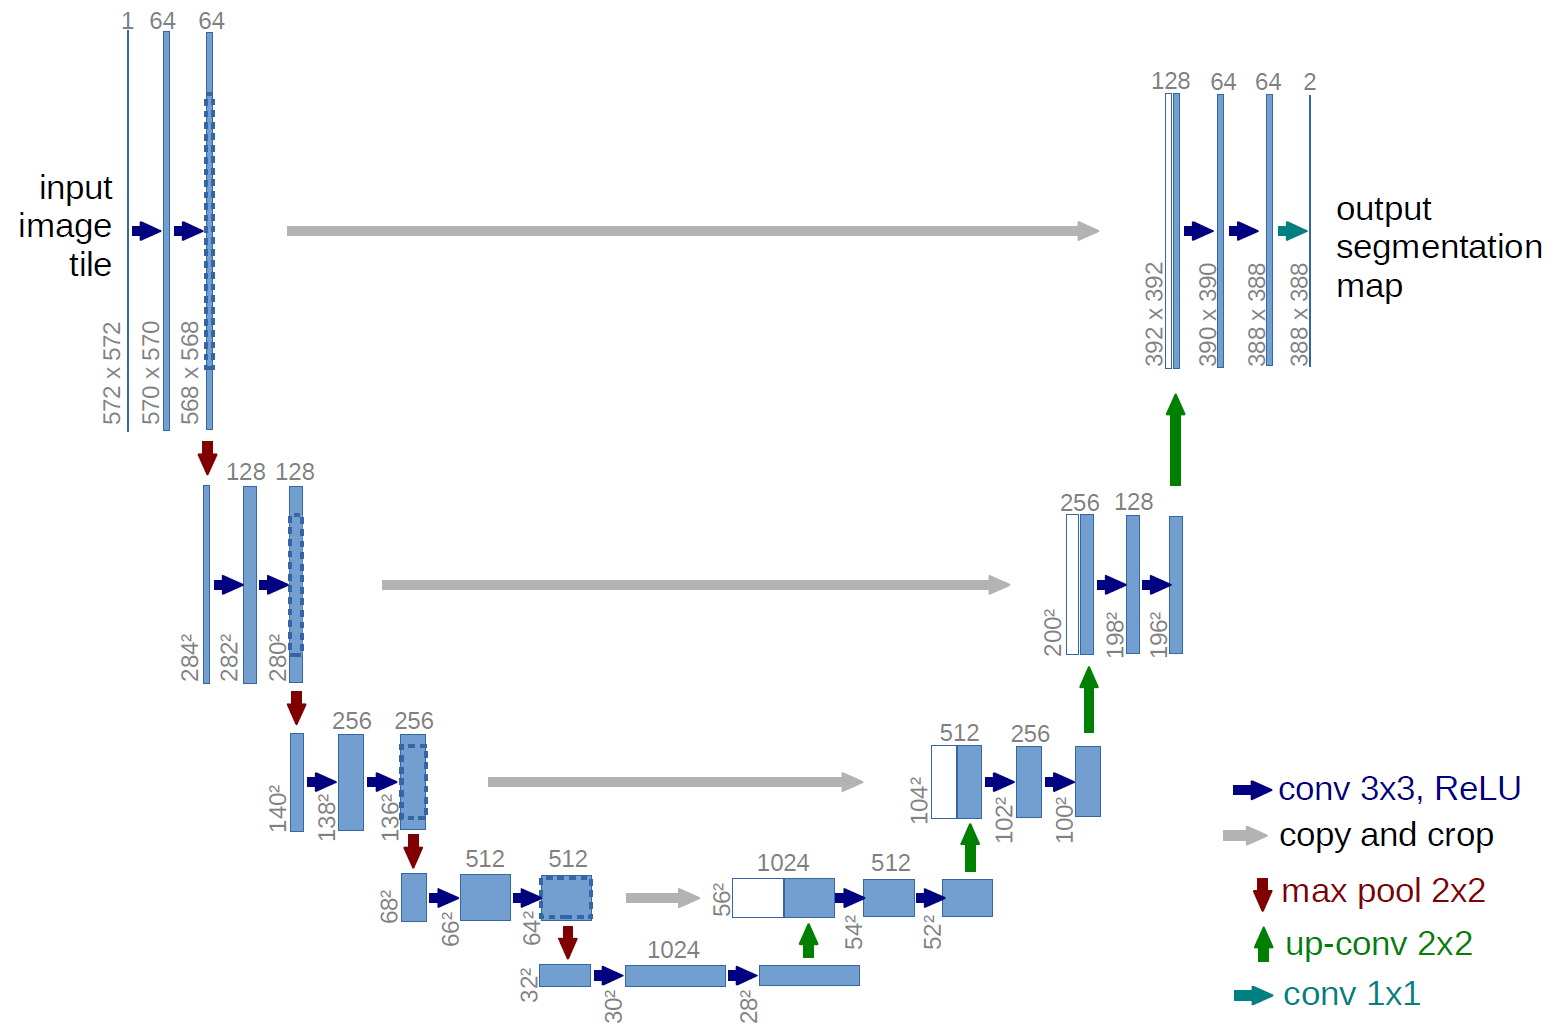
\includegraphics[width=0.5\textwidth]{figures/unet-architecture.png}
    \caption{U-Net Architecture~\cite{ronneberger2015u}}
    \label{fig:unet-architecture}
\end{figure}

The Feature Pyramid Network (FPN)~\cite{lin2017feature} shares part of its structure with the U-Net, except it explicitly combines the features of each upscaling layer to predict the final semantic segmentation mask as visualized in Figure~\ref{fig:fpn-architecture}. The main difference between FPN and U-Net is that FPN takes more time to process images. It does produce better results for smaller and medium-sized objects.

\begin{figure}[ht]
    \centering
    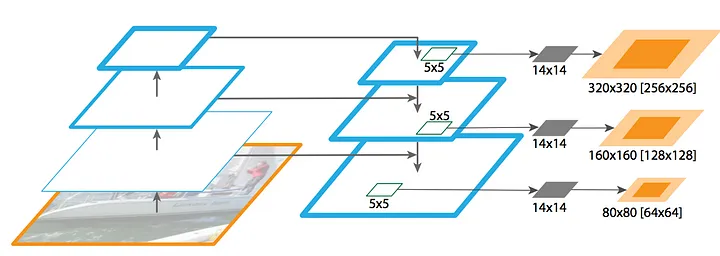
\includegraphics[width=0.5\textwidth]{figures/fpn-architecture.png}
    \caption{Feature Pyramid Network Architecture~\cite{lin2017feature}}
    \label{fig:fpn-architecture}
\end{figure}

These models are very adaptable as their various parts, such as encoders, can easily be replaced. Thus they can be modified to adapt to the limitations of mobile robotics, by employing lightweight and fast encoders. Moreover, during the BRaTS2018~\cite{menze2014multimodal} competition, it has been shown to be very competitive achieving second place~\cite{DBLP:journals/corr/abs-1809-10483}. Next to that, they also both employ an encoder-decoder structure, which is similar to the VAE. Thus resulting in a more representative comparison.

\paragraph{}
\todo{Rewrite + move this to future work}
Although the above models are not state-of-the-art anymore, they remain easy to train and do not require exotic tricks to make them work. Moreover, they have good inference speed and are architecturely similar to our proposed method. The primary issue with these models is their limited field of view, resulting in difficulty in relating parts of the image that are far apart. This can partially be combatted by making use of dilated convolutional layers, such as proposed by Gao~\cite{gao2023rethinking}. Or by the use of vision tranformers~\cite{dosovitskiy2021image}, which can relate pixels that are far apart in the input image. These vision tranformers have been used successfully in the segmentation task~\cite{xie2021segformer,chen2022vision}. However, due to the computational complexity in vision tranformers they are not yet suitable for real-time inference on mobile robotics. $TODO$ Reference to `no new-net', of why U-Net is good enough for our use-case.
Another impressive example is the Segment Anything Model (SAM)~\cite{kirillov2023segment}. It is a huge, and slow, network capable of, as the name implies, anything based on a prompt. Although not relevant for comparison, it can be used to aid the labour intensive task of labelling new data.


\chapter{Method}\label{chapter:first_real_chapter}
From a probabilistic point of view, semantic segmentation can be modelled as $p_\theta(x,y)$, where $x$ is a given (RGB-)image, and $y$ is the semantic label. However, in practice, there also exists $z$, the physical object of which $x$ is a view. Thus, we propose the probabilistic model to be $p_\theta(x,y,z)$, which can be rewritten as: $p_\theta(x,y,z)$ = $p_\theta(y|x,z) p_\theta(x|z) p_\theta(z)$.
\begin{itemize}
    \item $p_\theta(z)$; The generative process of the object.
    \item $p_\theta(x|z)$; The generative process of the observation of the object.
    \item $p_\theta(y|x,z)$; The generative process of the semantic meaning in the viewport of the observation.
\end{itemize}
Notice that the model $p_\theta(x|z) p_\theta(z)$ is equal to the VAE. We propose to first learn the generative model $p_\theta(x,z) = p_\theta(x|z) p_\theta(z)$, by learning the approximation of $p_\theta(x|z)$ and $p_\theta(z)$, using a VAE. After which we can use that learnt model to approximate the parameters of $p_\theta(y|x,z)$.

\section{Model}
We start by rewriting the log-likelihood of $p_\theta(x, y)$ as shown in Eq.~\ref{eq:p_x_y_rewrite}, a detailed derivation of this is shown in Appendix~\ref{appendix:full_derivation}. As the KL-divergence is $\geq 0$, the rest of the equation is the lower bound. Notice that the rest contains the $\mathcal{L}_ELBO$, which can be separated. This results in the equation $\mathcal{L}_{l-ELBO}$, shown in Eq.~\ref{eq:label_ELBO}. To be able to exert more control over the importance of each of the factors during training, we also introduce the $\mathcal{L}_{\beta\gamma l-ELBO}$, as shown in Eq.~\ref{eq:beta_label}.

\begin{subequations}
    \begin{align}
        \log p_\theta(x, y)
         & = D_{KL}(q_\phi(z|x) || p_\theta(z|x)) + \mathbb{E}_{q_{\phi}(z | x)}[\log p_\theta(x, y | z)] - D_{KL}(q_{\phi}(z|x) || p(z))  \label{eq:p_x_y_rewrite}                                                \\
         & \geq \mathbb{E}_{q_{\phi}(z | x)}[\log p_\theta(x, y | z)] - D_{KL}(q_{\phi}(z|x) || p(z))                                                                                                              \\
         & = \mathbb{E}_{q_{\phi}(z | x)}[\log p_\psi(y | x, z) + \log p(x | z)] - D_{KL}(q_{\phi}(z|x) || p(z))                                                                                                   \\
         & = \mathbb{E}_{q_{\phi}(z | x)}[\log p_\psi(y | x, z)] + \mathbb{E}_{q_{\phi}(z | x)}[\log p_\theta(x | z)] - D_{KL}(q_{\phi}(z|x) || p_\theta(z))                                                       \\
         & = \mathbb{E}_{q_{\phi}(z | x)}[\log p_\psi(y | x, z)] + \mathcal{L}_{ELBO}(\theta, \phi; x)                                                                                                             \\
         & = \mathcal{L}_{l-ELBO} \label{eq:label_ELBO}(\theta, \phi, \psi; x, z)                                                                                                                                  \\
        \mathcal{L}_{\beta\gamma l-ELBO}
         & = \mathbb{E}_{q_{\phi}(z | x)}[\log p_\psi(y | x, z)] + \gamma \cdot \mathbb{E}_{q_{\phi}(z | x)}[\log p_\theta(x | z)] - \beta \cdot D_{KL}(q_{\phi}(z|x) || p_\theta(z))        \label{eq:beta_label}
    \end{align}
\end{subequations}

Hence, we want to estimate the following three distributions using a neural network.
\begin{itemize}
    \item $q_\phi(z|x)$ (i.e., image encoder)
    \item $p_\theta(x|z)$ (i.e., image decoder)
    \item $p_\psi(y|x, z)$ (i.e., label decoder)
\end{itemize}
We will refer to the image encoder and label decoder together as VAE-Segmentation (VAES). A schematic of the model can be seen in Figure~\ref{fig:schematic-vaes}.

\begin{figure}[h]
    \centering
    \subfloat[A classic VAE and our model during the pre-training phase.\label{fig:schematic-vae}]{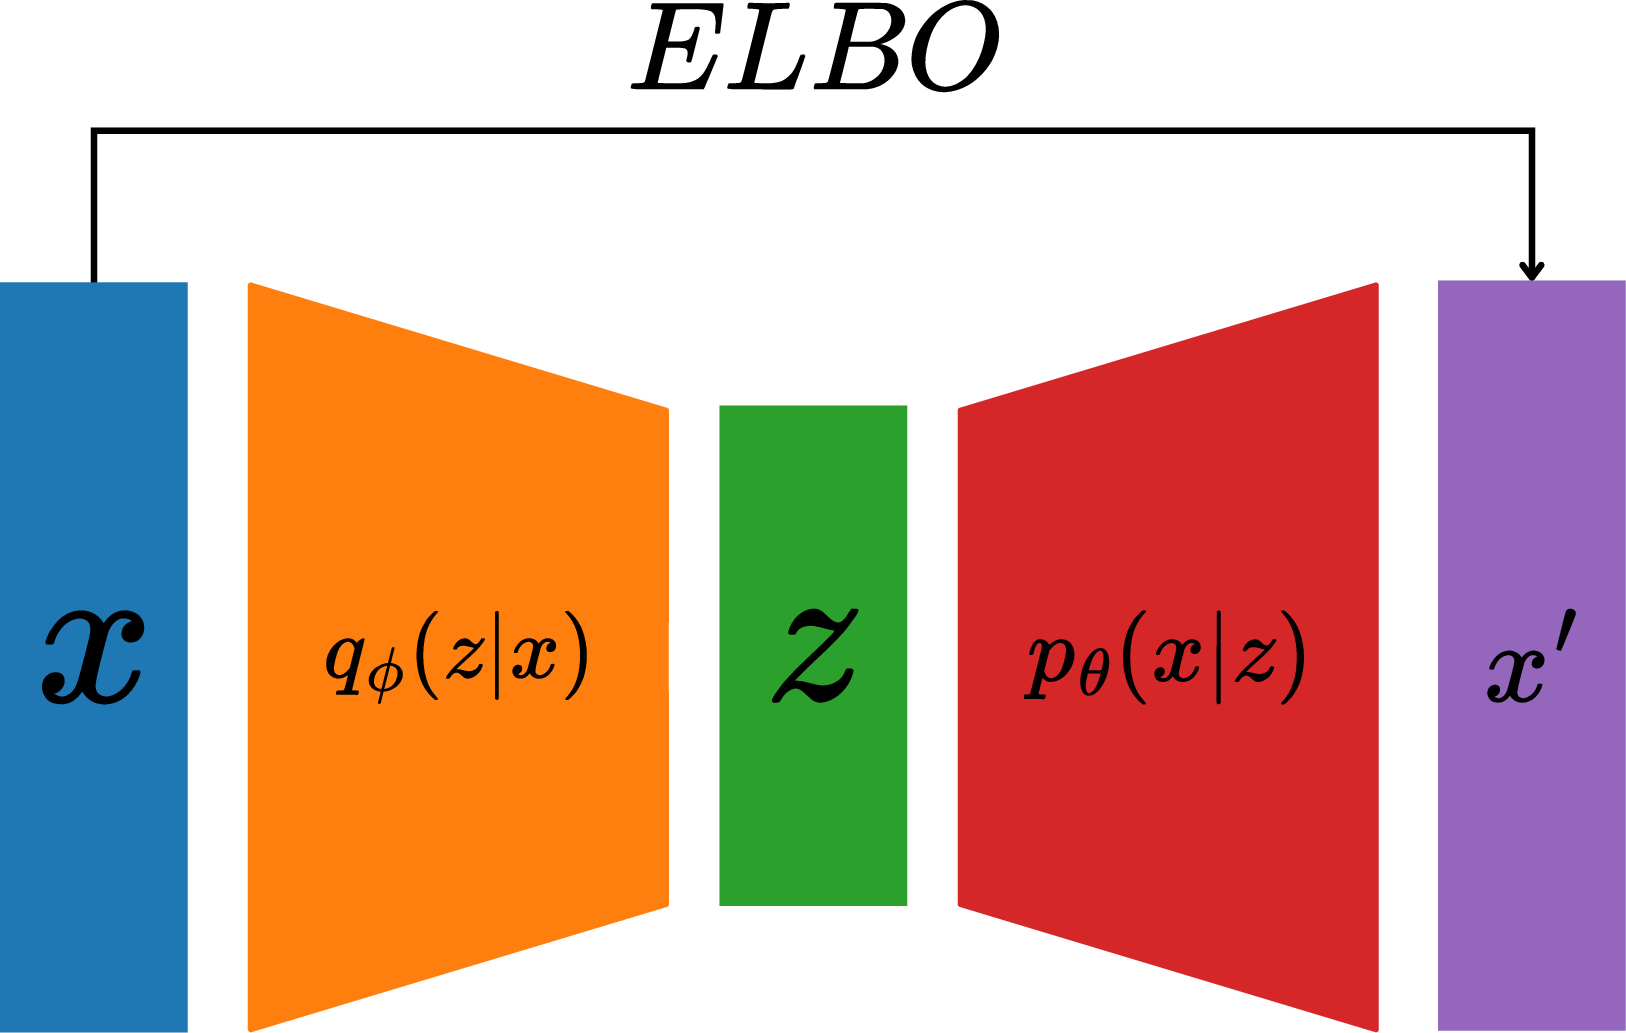
\includegraphics[width=0.45\textwidth]{figures/vae.png}}\hphantom{space}
    \subfloat[The full VAES model. The dotted line shows the skip connections. During inference the image decoder can be disregarded\label{fig:schematic-vaes}]{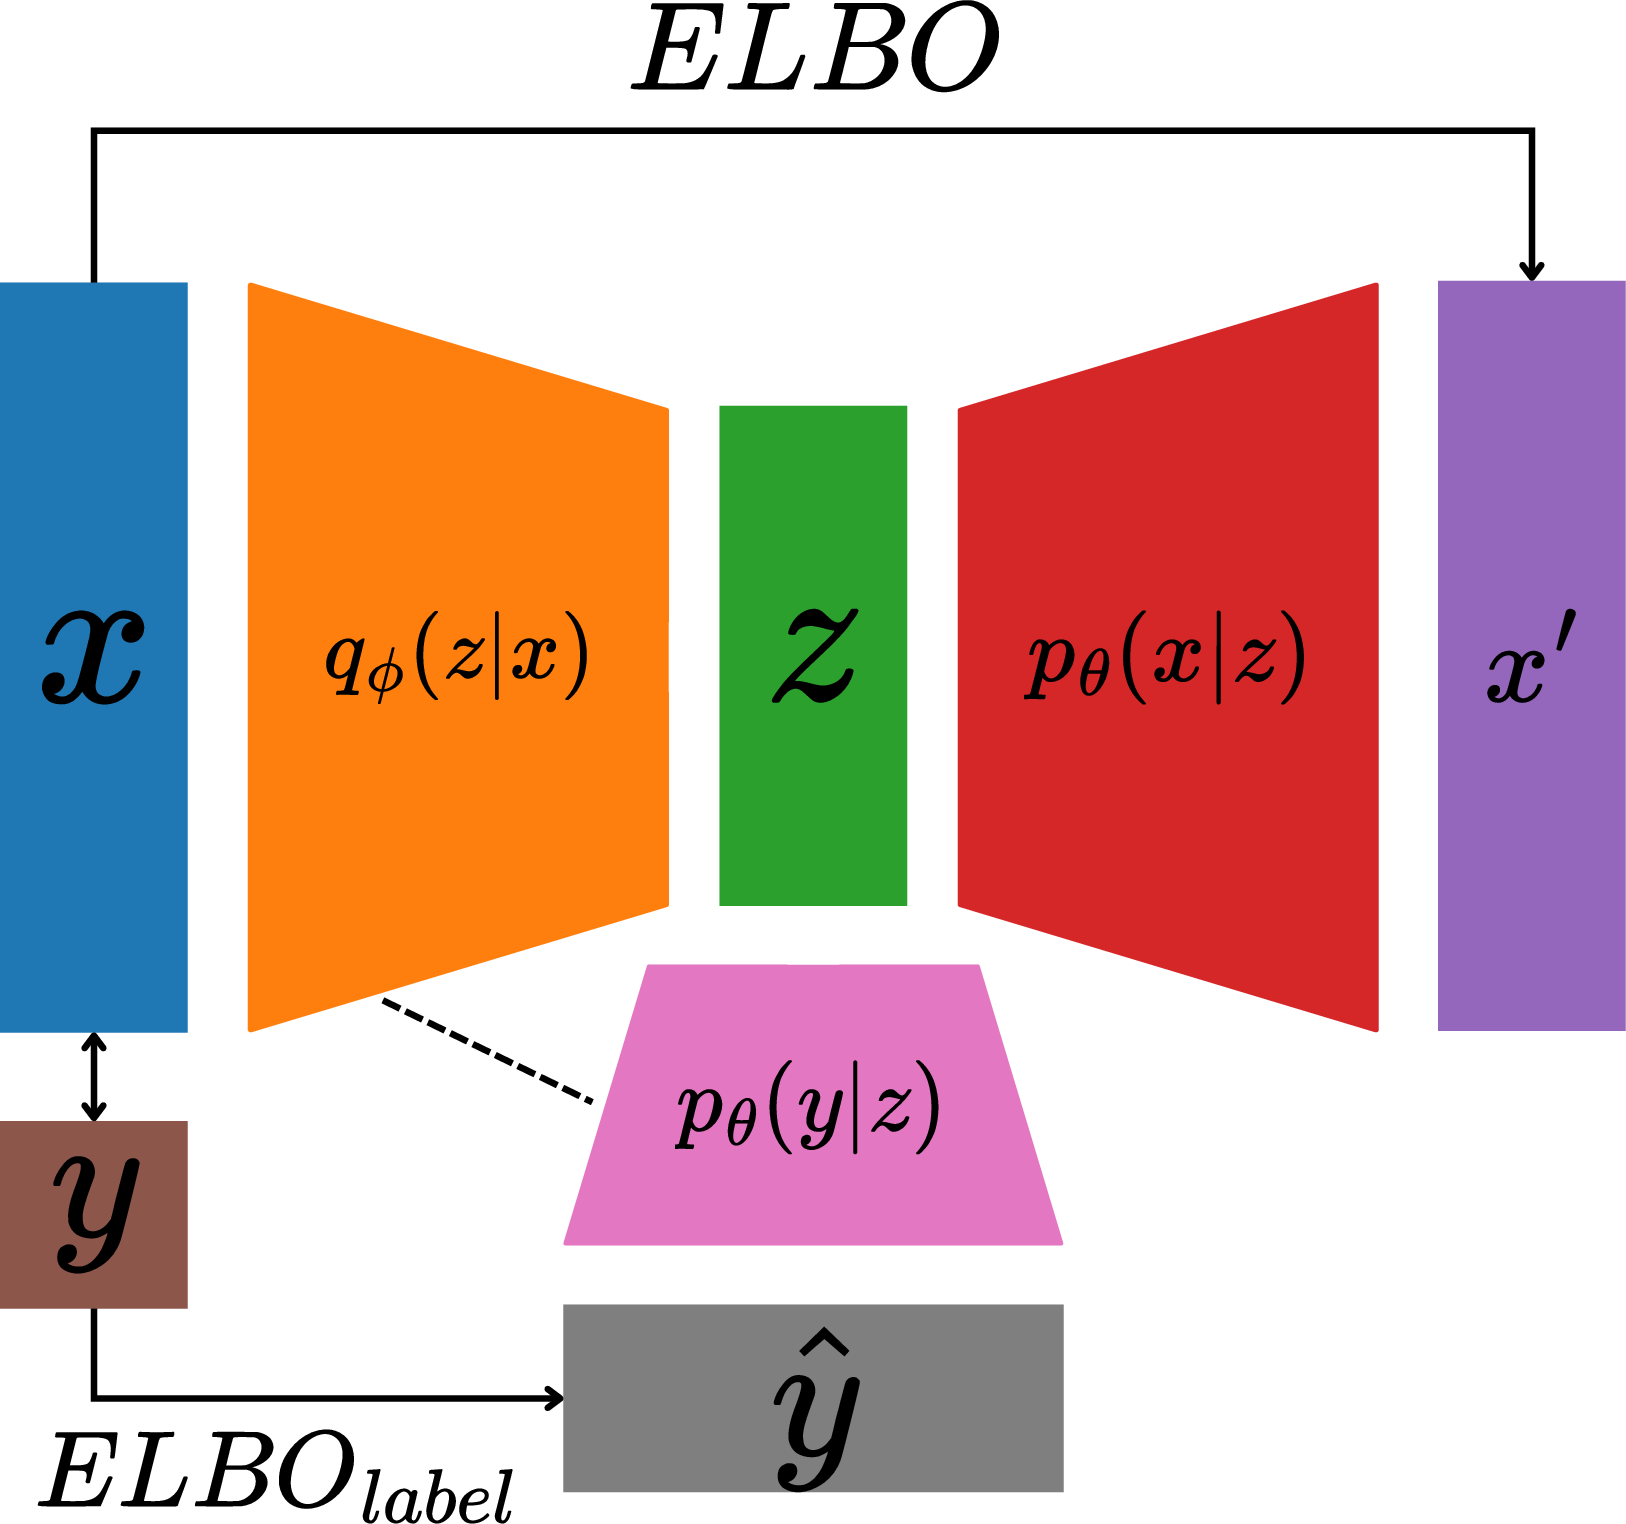
\includegraphics[width=0.45\textwidth]{figures/vaes.png}}
    \caption{A schematic of the proposed VAES.}
\end{figure}

\subsection{Image Encoder}
The image encoder approximates the latent distribution, $p_\theta(z)$. To ensure we can train the encoder using gradient descent, we need to make sure it is fully differentiable. Thus, we make use of the reparametrization trick. We use a deterministic mapping $g_\phi(\epsilon, z')$, where $\epsilon$ is an independent random variable and $g_\phi(x)$ is our (deterministic) neural network. Kingma et al.~\cite{kingma2014autoencodingvariationalbayes} show that by using this reparametrization trick a wide range of distributions can be learnt. In our case, we use a Gaussian latent space. The reparametrization then becomes $z = \mu + \sigma \epsilon$, where $\mu$ and $\sigma$ are the output of our image encoder network.

\subsection{Image Decoder}
The image decoder approximates the conditional Gaussian distribution $p_\theta(x|z)$. It is used during the pre-training step to prime the image encoder with 'good' initial weights, using the traditional ($\beta$-)VAE training. The hypothesis is, that given that $x$ can be reconstructed from the learnt $q_\phi(z|x)$, the learnt latent space contains useful features to approximate $p_\theta(y|x,z)$. In Eq.~\ref{eq:beta-elbo} $\log p_\theta(x|z)$ can be calculated using Eq.~\ref{eq:log_p_x_z} using a parameterized neural network.

\begin{equation}
    \begin{split}
        \log p_\theta(x|z)      & = \log \mathcal{N}(x; \mu, \sigma^2I) \label{eq:log_p_x_z} \\
        \text{where}~\mu,\sigma & =NN_\theta(z)
    \end{split}
\end{equation}

\subsection{Label Decoder}
The label decoder is similar to the image decoder, except that it approximates a multivariate Bernoulli distribution, instead of a Gaussian distribution. Thus, the calculation of $\log p_\theta(y|x,z)$ is different, which is shown in Eq.~\ref{eq:log_p_y_z}. Furthermore, it has `skip connections'. These skip connections allow for information to flow directly from a higher layer in the encoder to the decoder. We make the distinction between 3 types of skip connections.
\begin{enumerate}
    \item Skip: The output of the encoder layer is directly passed to the decoder.
    \item Projection: The output of the encoder layer is first projected using a convolutional layer.
    \item Variational: The output of the encoder layer is first projected using a variational convolutional layer.
\end{enumerate}
When all skip connections are of the type `Skip', our architecture is equal to the U-Net architecture.

\begin{subequations}
    \begin{align}
        \log p_\psi(y|x, z) & = \prod^C \sum_{i=0}^n y_{i,c} \log h_{i,c} \label{eq:log_p_y_z} \\
        \text{where}~h      & = \text{softmax}(NN_\theta(x, z))
    \end{align}
\end{subequations}

\section{Training procedure}
The training consists of two stages, the pre-training phase, and the fine-tuning stage. 
\paragraph*{Pre-training phase} During the pre-training phase, the image encoder, $q_\phi(z|x)$, and image decoder, $p_\theta(x|z)$, are trained according to Algorithm~\ref{alg:pre-training}. This algorithm is equal to the one proposed by Kingma et al.~\cite{kingma2014autoencodingvariationalbayes}. The model parts shown in Figure~\ref{fig:schematic-vae} are optimized.

\RestyleAlgo{ruled}
\begin{algorithm}
    \caption{Pre-training: The pre-training phase is equal to the AEVB, i.e., VAE, algorithm proposed by Kingma et al.~\cite{kingma2014autoencodingvariationalbayes}.}
    $\theta, \phi \gets$ Initialize parameters\;
    \Repeat{Convergence of $\theta, \phi$}{
        $\mathbf{X}^M \gets $ Sample a random minibatch of size $M$\;
        $g \gets \nabla_{\theta, \phi} \mathcal{L}_{ELBO} (\theta, \phi; \mathbf{X}^M)$ Calculate the gradients.\; 
        $\theta, \phi \gets$ Update parameters using gradients $g$ (E.g. using AdaMax\cite{kingma2017adammethodstochasticoptimization}) \;
    }
    \Return{$\theta, \phi$}
    \label{alg:pre-training}
\end{algorithm}


\paragraph*{Fine-tuning phase} During the fine-tuning phase, the learnt image encoder, $q_\phi(z|x)$, is reused. A new label decoder, $p_\psi(y|x, z)$, is initialized and optimized. The encoder can either be jointly optimized or kept frozen. Note that if we are not interested in the probability $p_\phi(x | z)$ and have chosen $\gamma = 0$ for $\mathcal{L}_{\beta\gamma l-ELBO}$, we can disregard it to reduce the computational load during training. The pseudocode can be seen in Algorithm~\ref{alg:fine-tuning}.

\begin{algorithm}
    \caption{Fine-tuning: The fine-tuning phase }
    $\theta, \phi \gets$ Initialize $\theta, \phi$ using the pre-training algorithm shown in Algorithm~\ref{alg:pre-training}\;
    $\psi \gets$ Initialize $\psi$\;
    \Repeat{Convergence of $\theta, \psi, \phi$}{
        $\mathbf{X}^M, \mathbf{Y}^M \gets $ Sample a random minibatch of size $M$\;
        $z^M \sim q_\phi(z | \mathbf{X}^M)$ Sample from the learnt encoder\;
        $g \gets \nabla_{\psi, \phi} \mathcal{L}_{l-ELBO} (\psi, \phi; \mathbf{X}^M, z^M)$ Calculate the gradients\;
        $\psi \gets$ Update $\psi$ using gradients $g$ (E.g. using AdaMax~\cite{kingma2017adammethodstochasticoptimization})\;
        \lIf{$\theta$ is not frozen}{$\theta \gets$ Update $\theta$ using gradients}
        \lIf{$\gamma \neq 0$}{$\phi \gets$ Update $\phi$ using gradients}
    }
    \Return{$\theta, \psi, \phi$}
    \label{alg:fine-tuning}
\end{algorithm}


\section{Evaluation}
\subsection{Inference}
Due to the variational architecture of the model, the inference can be done in two ways. One way is deterministic, by taking the mode of each latent vector. The other is variational, by sampling each latent vector. During training sampling the latent space is useful to improve the stability of training. However, during evaluation, it is preferred for the model to be deterministic. Hence, during evaluation, the mode of the latent space is used.

\subsection{Metrics}
The most well-known and widely-used metrics within classification are precision (Eq.~\ref{eq:precision}), recall (Eq.~\ref{eq:recall}), and F1-score (Eq.~\ref{eq:f1})~\cite{rijsbergen1979information}. The latter is a combination of precision and recall. Within the field of image segmentation the F1-score is also sometimes referred to as the Recognition Quality (RQ). In this, TP, FP, and FN refer to the True Positive, False Positive, and False Negative predictions per pixel. As our model always gives a prediction for each pixel, an FP in one class will always coincide with an FN in another class. Another common metric is the Jaccard Index (Eq.~\ref{eq:jaccard}), which is monotonically similar to the F1-score but weighs incorrect predictions more. As they are similar we will only report the Jaccard Index.

\begin{subequations}
    \begin{align}
        \text{Precision}     & = \frac{TP}{TP + FP} \label{eq:precision}                                               \\
        \text{Recall}        & = \frac{TP}{TP + FN} \label{eq:recall}                                                  \\
        F1 = \text{RQ}       & = 2 \cdot \frac{\text{Precision} \cdot \text{Recall}}{\text{Precision} + \text{Recall}} \\ 
                             & = \frac{TP}{\frac{1}{2} (FN + FP) + TP} \label{eq:f1}                                   \\
        \text{Jaccard Index} & = \frac{TP}{FN + FP + TP} \label{eq:jaccard}
    \end{align}
\end{subequations}


\chapter{Experimental Setup}\label{chapter:second_real_chapter}

\section{Implementation details}
\subsection{Dataset}
\paragraph{COCO~\cite{lin2015microsoftcococommonobjects}} is a publicly available dataset and has a multitude of labels. The semantic mask are extrated from the 2017 Panoptic annotations. This set contains more than 100k images that are densly annotated with both the semantic class and instance. There are a total of 133 different classes which belong to 27 `supercategories'. The four categories ``food'' and ``food-stuff'' and ``furniture'' and ``furniture-stuff'' were merged into ``food'' and ``furniture'' respectively, bringing the number of supercategories to 25. To speed up convergences, we will use these 25 classes. The distribution of the class labels can be seen in Figure \ref{fig:coco-class-distribution}. Some samples of the dataset can be seen in Figure \ref{fig:coco-samples}. More samples can be found in Appendix \ref{appendix:coco_samples}. 


\begin{figure}[h]
    \centering
    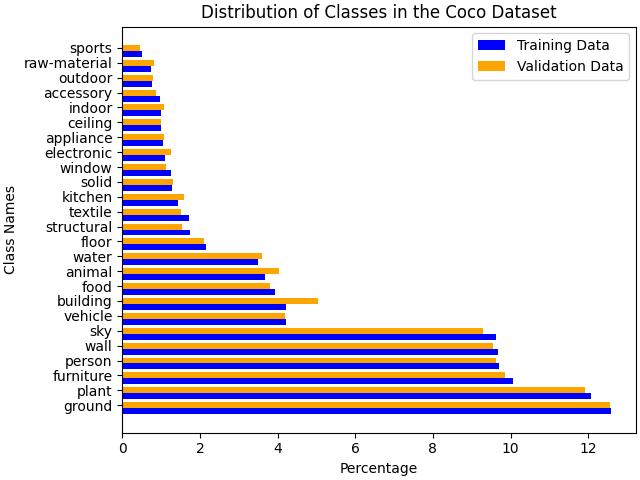
\includegraphics[width=0.9\textwidth]{figures/datasets/coco/class_distribution.png}
    \caption{Class Distribution of CoCo}
    \label{fig:coco-class-distribution}
\end{figure}

\begin{figure}
    \centering
    \subfloat[Training sample 0]{%
        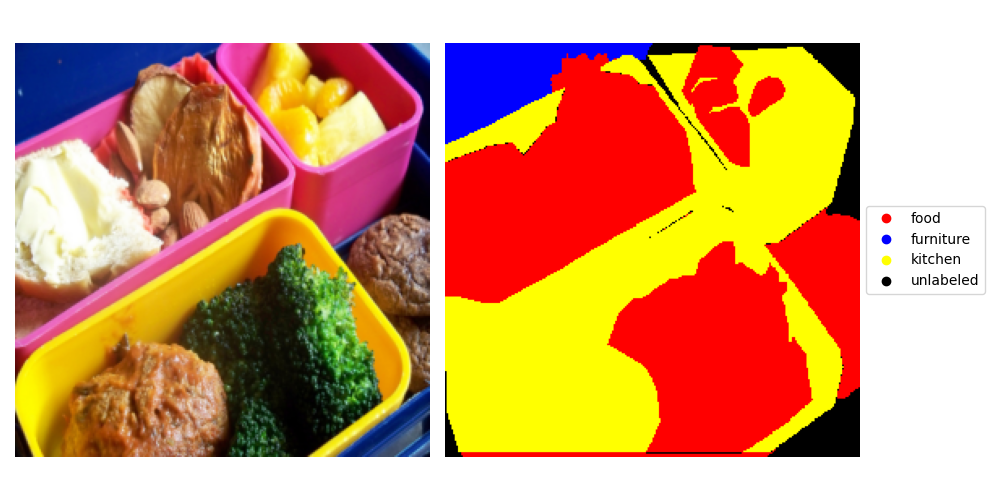
\includegraphics[width=0.5\textwidth]{figures/datasets/coco/samples/train/0.png}%
    }
    \subfloat[Training sample 1]{%
        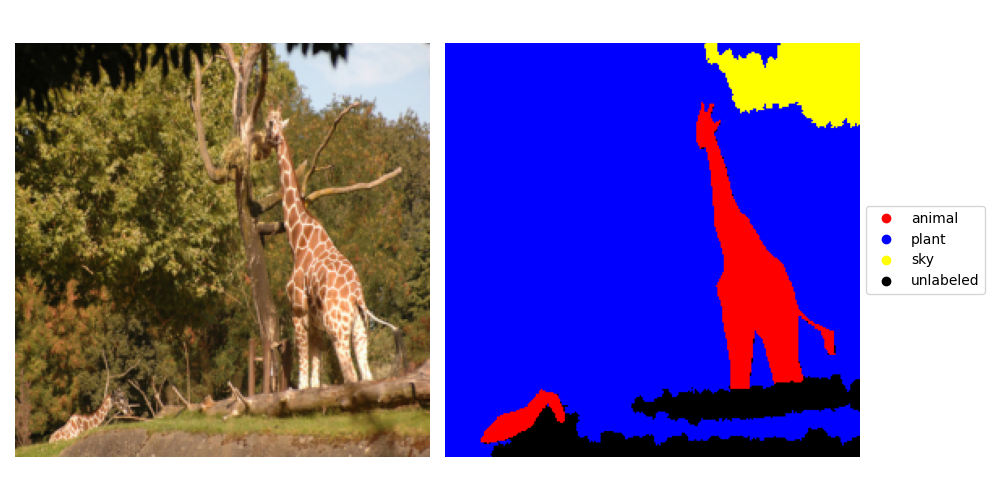
\includegraphics[width=0.5\textwidth]{figures/datasets/coco/samples/train/1.png}%
    }\\
    \subfloat[Validation sample 0]{%
        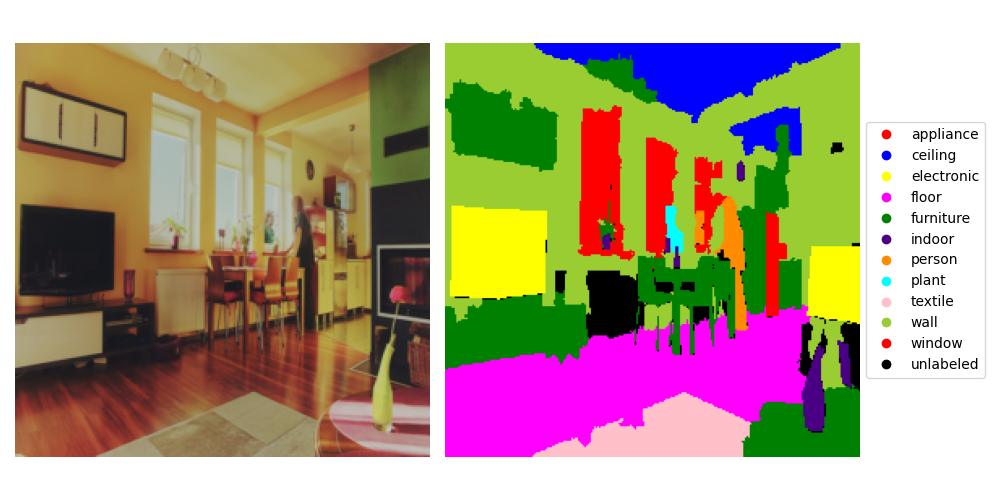
\includegraphics[width=0.5\textwidth]{figures/datasets/coco/samples/val/0.png}%
    }
    \subfloat[Validation sample 1]{%
        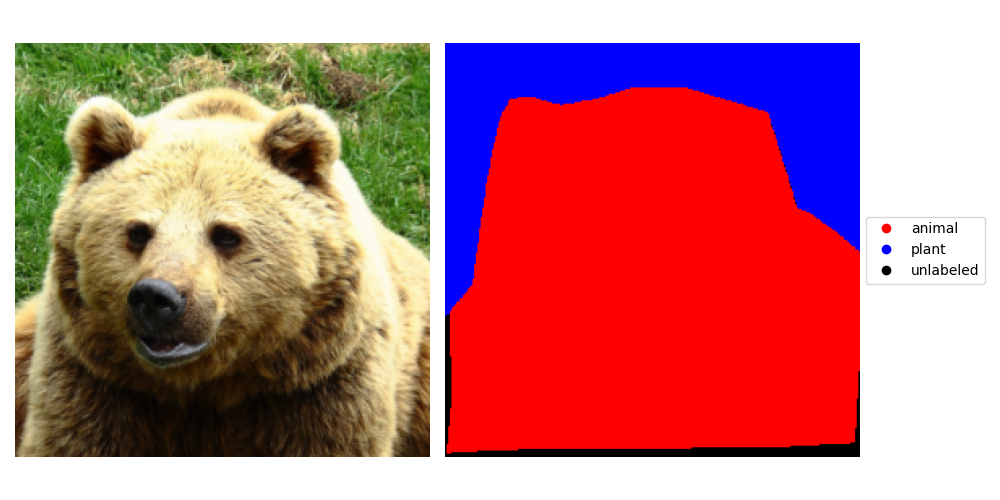
\includegraphics[width=0.5\textwidth]{figures/datasets/coco/samples/val/1.png}%
    }
    \caption{\label{fig:coco-samples}Ground truths for the dataset samples}
\end{figure}


\subsection{Training Settings}
All models are implemented in PyTorch~\cite{Ansel_PyTorch_2_Faster_2024} using an adapted version of the segmentation models repository~\cite{Iakubovskii:2019}. All code and configurations required to train the models and reproduce the experiments can be found on github \footnote[1]{\url{https://github.com/Generative-AI-TUe/msc-project-1297333}}. All models are trained on a NVIDIA Geforce RTX 2080 TI. The gradients are clipped using the norm, with a maximum value of 10. The AdaMax~\cite{kingma2017adammethodstochasticoptimization} is used with a cosine annealing learning rate, varying between $1e^{-3}$ and $1e^{-4}$. Each model is trained on 10.000 minibatches of size 96, unless otherwise specified.

\section{Comparison to baseline architectures}
For the experiments we make use of our method, VAES, FPN, and U-Net. Each model was trained eight times with different configurations. We used different settings for the pre-trained weights:
\begin{itemize}
    \item Without (`None') pre-trained weights.
    \item With pre-trained weights retrieved from classification of ImageNet.
    \item With pre-trained weights retrieved from a $\beta$-vae, with $\beta=1$ and $\beta=100$.
\end{itemize}
Additionally, the model is trained with `frozen' encoder weights (the encoder weights are not updated), and with `unfrozen' encoder weights (the encoder weights are updated). The resulting Evaluation Jaccard Index can be seen in Table~\ref{tab:baseline_results}.

\begin{table}[ht]
\centering
\caption{The Evaluation Jaccard Index for our model and the baselines for various parameters. The higher the score, the better.}
\label{tab:baseline_results}
\begin{tabular}{llrrrr}
\toprule
 & weights & None & imagenet & vae-b1 & vae-b100 \\
frozen & architecture &  &  &  &  \\
\midrule
\multirow[t]{3}{*}{False} & VAES & 0.21 & 0.47 & 0.20 & 0.15 \\
 & fpn & \textbf{0.30} & \textbf{0.52} & \textbf{0.26} & \textbf{0.28} \\
 & unet & 0.23 & 0.49 & 0.21 & 0.24 \\
\cline{1-6}
\multirow[t]{3}{*}{True} & VAES & n.a. & 0.40 & 0.20 & 0.18 \\
 & fpn & n.a. & 0.45 & 0.21 & 0.21 \\
 & unet & n.a. & 0.42 & 0.20 & 0.19 \\
\cline{1-6}
\bottomrule
\end{tabular}
\end{table}


An Analysis of Variance (ANOVA) is done, of which the results can be seen in Table~\ref{tab:comparison_baselines_anova_all}. Based on these results an Ordinary Least Squares Linear Model (OLS) is fitted to determine the effect of each significant parameter. The results of this are shown in Table~\ref{tab:comparison_baselines_ols_effects}.

\begin{figure}[h]
    \foreach \i in {0,1,...,4} {
            \centering
            \subfloat[Image]{\includegraphics[width=0.2\textwidth]{figures/baselines/samples/VAES-imagenet-False/\i.png}}
            \subfloat[Ground Truth]{\includegraphics[width=0.2\textwidth]{figures/baselines/samples/VAES-imagenet-False/gt_\i.png}}
            \subfloat[VAES-imagenet]{\includegraphics[width=0.2\textwidth]{figures/baselines/samples/VAES-imagenet-False/pr_\i.png}}
            \subfloat[unet-imagenet]{\includegraphics[width=0.2\textwidth]{figures/baselines/samples/unet-imagenet-False/pr_\i.png}}
            \subfloat[fpn-imagenet]{\includegraphics[width=0.2\textwidth]{figures/baselines/samples/fpn-imagenet-False/pr_\i.png}}
            \\
        }
    \caption{Samples of the validation dataset, with the ground truth and the prediction by the model. The encoder is not frozen.}\label{ref:baseline-sample-results-0}
\end{figure}

\begin{table}[ht]
\centering
\caption{ANOVA results estimating the influence of each parameter.\\Where: \\\hphantom{tabb}`weights' are the pretrained weights (or lack thereof) used.\\\hphantom{tabb}`architecture' is the model architecture used.\\\hphantom{tabb}'frozen' indicates whether the encoder was frozen\\\hphantom{tabb}$A$:$B$ is the interaction effect between $A$ and $B$}
\label{tab:comparison_baselines_anova_all}
\begin{tabular}{lrrrrr}
\toprule
 & df & sum\_sq & mean\_sq & F & PR(>F) \\
\midrule
frozen & 1.00 & 0.00 & 0.00 & 5.29 & 0.08 \\
weights & 3.00 & 0.25 & 0.08 & 175.48 & \textbf{0.00} \\
architecture & 2.00 & 0.01 & 0.01 & 12.69 & \textbf{0.02} \\
frozen:weights & 3.00 & 0.00 & 0.00 & 1.53 & 0.34 \\
frozen:architecture & 2.00 & 0.00 & 0.00 & 2.16 & 0.23 \\
weights:architecture & 6.00 & 0.00 & 0.00 & 0.64 & 0.70 \\
Residual & 4.00 & 0.00 & 0.00 & n.a. & n.a. \\
\bottomrule
\end{tabular}
\end{table}


\begin{table}[ht]
\centering
\caption{Coefficients of the OLS showing the influence of the hyperparameters on the Evaluation Jaccard Index.\\Where:\\\hphantom{tabb}Coef. is the effectsize.\\\hphantom{tabb}P> |t| is the $p$-value. Bolded if significant ($\alpha\le0.05$).}
\label{tab:comparison_baselines_ols_effects}
\begin{tabular}{lrrrrrr}
\toprule
 & Coef. & Std.Err. & t & P>|t| & [0.025 & 0.975] \\
\midrule
Intercept & 0.22 & 0.02 & 10.54 & \textbf{0.00} & 0.17 & 0.26 \\
weights[T.imagenet] & 0.21 & 0.02 & 9.59 & \textbf{0.00} & 0.17 & 0.26 \\
weights[T.vae-b1] & -0.03 & 0.02 & -1.33 & 0.20 & -0.08 & 0.02 \\
weights[T.vae-b100] & -0.03 & 0.02 & -1.54 & 0.14 & -0.08 & 0.01 \\
architecture[T.fpn] & 0.06 & 0.02 & 3.49 & \textbf{0.00} & 0.02 & 0.09 \\
architecture[T.unet] & 0.02 & 0.02 & 1.48 & 0.16 & -0.01 & 0.06 \\
\bottomrule
\end{tabular}
\end{table}


\section{Reduction data required}
To determine if pre-training results in a reduction of labeled training data required, a full factorial design is done over the parameters: architecture type, pre-trained weights, and the percentage of the (labeled) dataset used. The resulting Evaluation Jaccard Index of each model configuration can be seen in Table~\ref{tab:data_fraction_results} and are plotted in Figure~\ref{fig:dataset-fraction-results}.
\begin{table}[ht]
\centering
\caption{The Evaluation Jaccard Index for the various models and dataset fractions. The higher the score the better.}
\label{tab:data_fraction_results}
\begin{tabular}{llrrrr}
\toprule
 & fraction & 1.000000 & 0.100000 & 0.010000 & 0.001000 \\
architecture & weights &  &  &  &  \\
\midrule
\multirow[c]{3}{*}{VAES} & None & 0.15 & 0.16 & 0.18 & 0.12 \\
 & imagenet & 0.34 & 0.37 & 0.39 & 0.21 \\
 & vae-b10 & 0.14 & 0.16 & 0.18 & 0.12 \\
\multirow[c]{3}{*}{fpn} & None & 0.22 & 0.12 & 0.21 & 0.17 \\
 & imagenet & 0.45 & \textbf{0.48} & \textbf{0.48} & \textbf{0.34} \\
 & vae-b10 & 0.19 & 0.21 & 0.23 & 0.16 \\
\multirow[c]{3}{*}{unet} & None & 0.21 & 0.10 & 0.18 & 0.14 \\
 & imagenet & \textbf{0.46} & 0.44 & 0.43 & 0.30 \\
 & vae-b10 & 0.20 & 0.18 & 0.21 & 0.14 \\
\bottomrule
\end{tabular}
\end{table}


\begin{figure}[h]
    \centering
    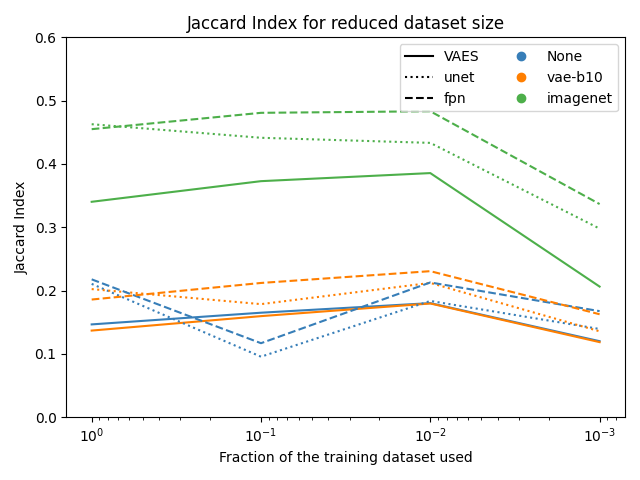
\includegraphics[width=0.9\textwidth]{figures/data_percentage/line-plot.png}
    \caption{Jaccard Index for reduced training dataset size.}
    \label{fig:dataset-fraction-results}
\end{figure}

An Analysis of Variance (ANOVA) is done, of which the results can be seen in Table~\ref{tab:data_fraction_parameter_significance}. Based on these results, it can be determined that there are no significant interaction effects between any of the parameters, and that each individual parameter has a significant effect.
\begin{table}[ht]
\centering
\caption{Anova results estimating the influence of each parameter.\\Where: \\\hphantom{tabb}`weights' are the pretrained weights (or lack thereof) used.\\\hphantom{tabb}`architecture' is the model architecture used.\\\hphantom{tabb}`$\log_{10}(\text{fraction})$' is the fraction of data used in log scale.\\\hphantom{tabb}$A$:$B$ is the interaction effect between $A$ and $B$}
\label{tab:data_fraction_parameter_significance}
\begin{tabular}{lrrrrr}
\toprule
 & df & sum\_sq & mean\_sq & F & PR(>F) \\
\midrule
weights & 2.00 & 0.39 & 0.20 & 75.49 & \textbf{0.00} \\
architecture & 2.00 & 0.02 & 0.01 & 4.61 & \textbf{0.02} \\
weights:architecture & 4.00 & 0.01 & 0.00 & 0.93 & 0.47 \\
$\log_{10}(\text{fraction})$ & 1.00 & 0.02 & 0.02 & 6.45 & \textbf{0.02} \\
$\log_{10}(\text{fraction})$:weights & 2.00 & 0.01 & 0.01 & 2.11 & 0.15 \\
$\log_{10}(\text{fraction})$:architecture & 2.00 & 0.00 & 0.00 & 0.22 & 0.80 \\
$\log_{10}(\text{fraction})$:weights:architecture & 4.00 & 0.00 & 0.00 & 0.01 & 1.00 \\
Residual & 18.00 & 0.05 & 0.00 & n.a. & n.a. \\
\bottomrule
\end{tabular}
\end{table}


The effect of the parameters can then be analysed by a simple OLS model. The results of which are shown in Table~\ref{tab:data_fraction_parameter_influence}. It shows that there is a large and significant increase in performance when using the ImageNet weights. The weights gained from pre-training a VAE do not significantly affect the performance, compared to random weights. Furthermore, both the FPN and UNet architectures are better than the VAES architecture. Finally, the size of the dataset is significant, however it is more important to choose the right architecture and especially pre-trained weights.
\begin{table}
    \centering
    \caption{Coefficients of the OLS.\\Where:\\\hphantom{tabb}Coef. is the effectsize.\\\hphantom{tabb}P> |t| is the $p$-value. Bolded if significant ($\alpha\leq0.05$).}
    \label{tab:data_fraction_parameter_influence}
    \begin{tabular}{lrrrrrr}
        \toprule
                                     & Coef. & Std.Err. & t     & P>|t|         & [0.025 & 0.975] \\
        \midrule
        Intercept                    & 0.16  & 0.02     & 7.56  & \textbf{0.00} & 0.12   & 0.20   \\
        weights[T.imagenet]          & 0.23  & 0.02     & 11.66 & \textbf{0.00} & 0.19   & 0.27   \\
        weights[T.vae-b10]           & 0.01  & 0.02     & 0.67  & 0.50          & -0.03  & 0.05   \\
        architecture[T.fpn]          & 0.06  & 0.02     & 3.19  & \textbf{0.00} & 0.02   & 0.10   \\
        architecture[T.unet]         & 0.04  & 0.02     & 2.05  & \textbf{0.05} & 0.00   & 0.08   \\
        $\log_{10}(\text{fraction})$ & 0.02  & 0.01     & 2.71  & \textbf{0.01} & 0.00   & 0.03   \\
        \bottomrule
    \end{tabular}
\end{table}


\section{Model Characteristics}

As the computational resources in mobile robots tend to be low, the inference speed and memory usage was measured. Inference was done on a NVIDIA GTX 1070, and measured using PyTorch benchmarking tools. The results can be seen in Table~\ref{tab:model_characteristics}.

\begin{longtable}[ht]{lrrrrrrrrrr}
\caption{Characteristics of the various architectures with ResNet50 as backbone. Inference measurements were done on a NVIDIA GTX 1070.} \label{tab:model_characteristics} \\
\toprule
 & Parameters ($1e^6$) & Total MAC ($1e^9$) & \multicolumn{4}{r}{Inference Speed (ms)} & \multicolumn{4}{r}{Memory Usage (mb)} \\
 &   &   & 1 & 2 & 8 & 32 & 1 & 2 & 8 & 32 \\
Name &  &  &  &  &  &  &  &  &  &  \\
\midrule
\endfirsthead
\caption[]{Characteristics of the various architectures with ResNet50 as backbone. Inference measurements were done on a NVIDIA GTX 1070.} \\
\toprule
 & Parameters ($1e^6$) & Total MAC ($1e^9$) & \multicolumn{4}{r}{Inference Speed (ms)} & \multicolumn{4}{r}{Memory Usage (mb)} \\
 &   &   & 1 & 2 & 8 & 32 & 1 & 2 & 8 & 32 \\
Name &  &  &  &  &  &  &  &  &  &  \\
\midrule
\endhead
\midrule
\multicolumn{11}{r}{Continued on next page} \\
\midrule
\endfoot
\bottomrule
\endlastfoot
vaes & 82.70 & 5.28 & 15.71 & 14.87 & 28.46 & 70.84 & 755.95 & 760.34 & 779.35 & 1062.98 \\
unet & 32.52 & 2.72 & 10.20 & 10.02 & 16.71 & 49.66 & \textbf{549.91} & \textbf{554.11} & \textbf{579.54} & \textbf{770.77} \\
fpn & \textbf{26.12} & \textbf{1.95} & \textbf{9.57} & \textbf{9.65} & \textbf{15.44} & \textbf{47.06} & 602.86 & 606.14 & 634.45 & 904.72 \\
\end{longtable}



\section{Ablation Study}
\subsection{Backbone}
We first analyse the influence of the backbone on the performance of the VAE task by comparing the following backbones: MobileViT~\cite{Mehta2022SeparableSF}, MobileNetV2~\cite{sandler2019mobilenetv2invertedresidualslinear}, EfficientNet~\cite{tan2020efficientnetrethinkingmodelscaling} and ResNet50~\cite{he2015deep}. The results can be seen in Table~\ref{tab:backbones-results}. Some examples of the reconstruction capabilities can be seen in Figure~\ref{fig:vae-backbones}.

\begin{figure}[!ht]
    \centering
    \caption{Example reconstruction for the various backbones.}
    \label{fig:vae-backbones}
    \subfloat[Original, EfficientNet]{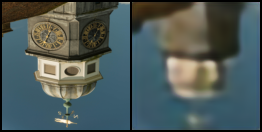
\includegraphics[width=0.45\linewidth]{figures/vae-backbones/samples/efficientnet_b2/4.png}}
    \subfloat[Original, MobileNetV2]{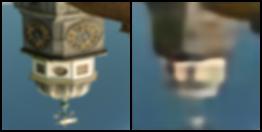
\includegraphics[width=0.45\linewidth]{figures/vae-backbones/samples/mobilenetv2_100/4.png}} \quad
    \subfloat[Original, MobileViT]{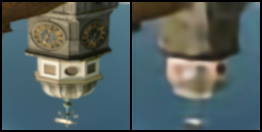
\includegraphics[width=0.45\linewidth]{figures/vae-backbones/samples/mobilevitv2_100/4.png}}
    \subfloat[Original, ResNet50]{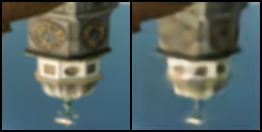
\includegraphics[width=0.45\linewidth]{figures/vae-backbones/samples/resnet50/4.png}}
\end{figure}

\begin{table}[ht]
\centering
\caption{VAE results of the various backbones.}
\label{tab:backbones-results}
\begin{tabular}{lrrrrr}
\toprule
 & Parameters ($1e^6$) & MAC ($1e^9$) & L1Loss (Recon) & KL-Divergence & Loss \\
Backbone &  &  &  &  &  \\
\midrule
MobileViT & 8.55 & 1.32 & 388158.31 & 5906.05 & 2402.00 \\
MobileNetV2 & \textbf{4.21} & \textbf{0.70} & 431505.41 & \textbf{5436.90} & 2774.02 \\
EfficientNet & 9.79 & 0.83 & 382322.31 & 16659.25 & 2911.08 \\
ResNet50 & 40.91 & 2.80 & \textbf{315560.38} & 9379.99 & \textbf{1792.29} \\
\bottomrule
\end{tabular}
\end{table}



\subsection{$\beta\text{-value}$}
We also analyse the effect of the $\beta$ factor on the reconstruction quality of the VAE. This is done by training models with varying values for $\beta$. The results can be seen in Table~\ref{tab:beta-vae-loss-values}. Some examples of the reconstruction capabilities can be seen in Figure~\ref{fig:beta-vae-recon-examples}. More samples can be seen in Appendix~\ref{appendix:recon_samples}.

\begin{table}[!ht]
    \centering
    \caption{Loss values resulting from training a Beta-VAE for various $\beta$ values}
    \label{tab:beta-vae-loss-values}
    \begin{tabular}{ccc}
        \hline
        $\beta$ & KL-Divergence & Reconstruction Error ($1e^5$) \\
        \hline
        0.01    & 80200         & 1.9                           \\
        0.1     & 31250         & 1.5                           \\
        1       & 8190          & 2.7                           \\
        10      & 2089          & 2.2                           \\
        100     & 498           & 2.9                           \\
        \hline
    \end{tabular}
\end{table}

\begin{figure}[!ht]
    \centering
    \caption{Example reconstructions for $\beta$-vae.}
    \label{fig:beta-vae-recon-examples}
    \subfloat[Original, $\beta$ = 0.01]{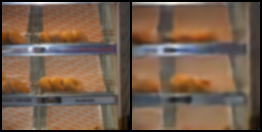
\includegraphics[width=0.45\linewidth]{figures/beta-vae/b0.01-0.png}}
    \subfloat[Original, $\beta$ = 0.1]{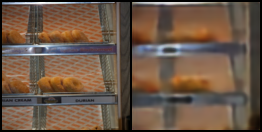
\includegraphics[width=0.45\linewidth]{figures/beta-vae/b0.1-0.png}} \quad
    \subfloat[Original, $\beta$ = 1]{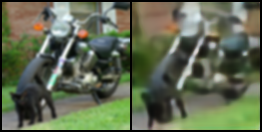
\includegraphics[width=0.45\linewidth]{figures/beta-vae/b1-0.png}}
    \subfloat[Original, $\beta$ = 10]{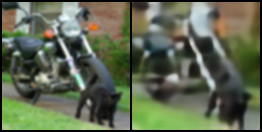
\includegraphics[width=0.45\linewidth]{figures/beta-vae/b10-0.png}}
\end{figure}


\subsection{Skip Connection}
To understand the importance of the type and amount of skip connections which are added after the pretraining, we will show the effect of this by incrementally removing more skip connections. We vary the amount of skip connections from 1 to 5 and try all 3 skip connection types. The results can be viewed in Table~\ref{tab:skip_results}
Again an ANOVA is fitted to determine the significant effects, the results can be seen in Table~\ref{tab:skip_importance_anova_all}. Then, an OLS is fitted to show the effect size of all significant factors, the results of which can be seen in Table~\ref{tab:skip_importance_ols_effects}. Neither the amount, nor type of skip connection matter significantly for the 

\begin{table}[ht]
\centering
\caption{Evaluation Jaccard Index for the VAES using different amounts and types of skip connections.}
\label{tab:skip_results}
\begin{tabular}{llrrr}
\toprule
 & skip\_type & proj & skip & var \\
 & skip\_num &  &  &  \\
\midrule
\multirow[c]{5}{*}{Evaluation Jaccard Index} & 1 & 0.412 & \textbf{0.426} & 0.410 \\
 & 2 & \textbf{0.462} & 0.452 & 0.429 \\
 & 3 & 0.474 & \textbf{0.493} & 0.463 \\
 & 4 & 0.456 & \textbf{0.494} & 0.434 \\
 & 5 & 0.440 & \textbf{0.490} & 0.433 \\
\multirow[c]{5}{*}{Parameters (x$1e^6$)} & 1 & 70.275 & \textbf{32.525} & 108.026 \\
 & 2 & 79.714 & \textbf{32.525} & 126.903 \\
 & 3 & 82.073 & \textbf{32.525} & 131.622 \\
 & 4 & 82.663 & \textbf{32.525} & 132.802 \\
 & 5 & 82.700 & \textbf{32.525} & 132.876 \\
\multirow[c]{5}{*}{Total MAC (x$1e^9$)} & 1 & 3.319 & \textbf{2.715} & 3.923 \\
 & 2 & 3.923 & \textbf{2.715} & 5.131 \\
 & 3 & 4.527 & \textbf{2.715} & 6.340 \\
 & 4 & 5.132 & \textbf{2.715} & 7.548 \\
 & 5 & 5.283 & \textbf{2.715} & 7.851 \\
\bottomrule
\end{tabular}
\end{table}


\begin{table}[ht]
\centering
\caption{ANOVA results estimating the influence of each parameter.\\Where: \\\hphantom{tabb}`weights' are the pretrained weights (or lack thereof) used.\\\hphantom{tabb}`architecture' is the model architecture used.\\\hphantom{tabb}'frozen' indicates whether the encoder was frozen\\\hphantom{tabb}$A$:$B$ is the interaction effect between $A$ and $B$}
\label{tab:comparison_baselines_anova_all}
\begin{tabular}{lrrrrr}
\toprule
 & df & sum\_sq & mean\_sq & F & PR(>F) \\
\midrule
frozen & 1.00 & 0.00 & 0.00 & 5.29 & 0.08 \\
weights & 3.00 & 0.25 & 0.08 & 175.48 & \textbf{0.00} \\
architecture & 2.00 & 0.01 & 0.01 & 12.69 & \textbf{0.02} \\
frozen:weights & 3.00 & 0.00 & 0.00 & 1.53 & 0.34 \\
frozen:architecture & 2.00 & 0.00 & 0.00 & 2.16 & 0.23 \\
weights:architecture & 6.00 & 0.00 & 0.00 & 0.64 & 0.70 \\
Residual & 4.00 & 0.00 & 0.00 & n.a. & n.a. \\
\bottomrule
\end{tabular}
\end{table}


\begin{table}[ht]
\centering
\caption{Coefficients of the OLS showing the influence of the hyperparameters on the Evaluation Jaccard Index.\\Where:\\\hphantom{tabb}Coef. is the effectsize.\\\hphantom{tabb}P> |t| is the $p$-value. Bolded if significant ($\alpha\le0.05$).}
\label{tab:comparison_baselines_ols_effects}
\begin{tabular}{lrrrrrr}
\toprule
 & Coef. & Std.Err. & t & P>|t| & [0.025 & 0.975] \\
\midrule
Intercept & 0.22 & 0.02 & 10.54 & \textbf{0.00} & 0.17 & 0.26 \\
weights[T.imagenet] & 0.21 & 0.02 & 9.59 & \textbf{0.00} & 0.17 & 0.26 \\
weights[T.vae-b1] & -0.03 & 0.02 & -1.33 & 0.20 & -0.08 & 0.02 \\
weights[T.vae-b100] & -0.03 & 0.02 & -1.54 & 0.14 & -0.08 & 0.01 \\
architecture[T.fpn] & 0.06 & 0.02 & 3.49 & \textbf{0.00} & 0.02 & 0.09 \\
architecture[T.unet] & 0.02 & 0.02 & 1.48 & 0.16 & -0.01 & 0.06 \\
\bottomrule
\end{tabular}
\end{table}



\chapter{Conclusions}\label{chapter:conclusions}

This part still needs some expanding but my current conclusions can be boiled down to the following bullet-points:
\begin{itemize}
    \item The VAE can be adapted for image segmentation, and works similarly to the UNet in prediction performance.
    \item In the context of mobile robotics there are some downsides compared to the classic UNet and FPN, as these are faster for inference.
    \item Skip connections do not seem to matter a lot.
    \item Pretraining using a VAE on the same dataset does not seem to beneficial, however importantly it is not detremental either. Thus it might be worth it to check if pretraining VAE on e.g. ImageNet does provide a benefit
\end{itemize}

\chapter{Future Work}\label{chapter:future_work}

\section{Improving VAES}
As already stated in the background section~\ref{chapter:background}, the VAE has some flaws that have been shown to be mitigable. We will highlight some interesting research that could be adapted to our method to possibly improve the quality of predictions.

\subsection{Larger dataset}
In this thesis, the pre-training of the VAES has been limited to the COCO~\cite{lin2015microsoftcococommonobjects} ($\sim$100k) dataset. However, similar to transformers, it might be beneficial to pre-train on larger datasets, such as OpenImagesV7~\cite{OpenImages} ($\sim$9M).

\subsection{Improving the Backbone}
One of the drawbacks of Fully Convolutional Network (FCN), is that in their classic form, as used by us, they have a small Field of View. This means they cannot relate parts of the image that are far apart. This can partially be combatted by making use of dilated convolutional layers, as proposed by Gao~\cite{gao2023rethinking}, or by the use of vision transformers~\cite{dosovitskiy2021image}, which can relate pixels that are far apart in the input image by leveraging attention mechanisms. These vision transformers have been used successfully in the segmentation task~\cite{xie2021segformer,chen2022vision}. However, they have two major drawbacks. One, as transformers have a lower inductive bias for vision~\cite{dosovitskiy2021image} compared to convolutional networks, they require much more data and time to train. Secondly, their attention mechanisms are computationally more complex than convolutional layers, thus they are more difficult to optimize for edge devices such as those required for mobile robotics. The first drawback can be countered by using publicly available pre-trained models. The second problem is more fundamental, and although there is research into making transformers more efficient~\cite{li2022efficientformer,Yu2021MetaFormerIA}, they remain more computationally expensive compared to their CNN counterparts.

\subsection{Improving the Sharpness}
Some reconstructed samples clearly show the disappearing of key features for semantic segmentation. This problem could potentially be mitigated by using different loss functions that focus more on the details. Or by the use of better architectures, such as the H-VAEs discussed in Chapter~\ref{chapter:background}, which improve the sharpness and reconstruction capabilities of the VAE.

\section{Extending VAES}
Next to the possibilities to mitigate current problems, VAEs can also be extended to provide additional benefits compared to the more classic discriminative approaches. In this section, we will highlight some possible extensions.

\subsection{Anomaly detection}
VAEs have been shown to be able to provide rudimentary anomaly detection. There are two prominent methods for this. The first method is by detecting unusual latent variables from the approximate posterior output $q_{\phi}(z|x)$~\cite{marimont2020anomalydetectionlatentspace,angiulli2020improving,angiulli2023latent}. The second method is by calculating the reconstruction error from the given input~\cite{an2015variational, zhou2020unsupervisedanomalylocalizationusing, gouda2022unsupervised}. The main benefit of the first method is that the decoder is not required for anomaly detection, resulting in a lower inference cost. In the case of robotics, it is important to detect unusual situations as it might result in unexpected behaviour which in turn could lead to dangerous situations. Therefore, it would be interesting to see if our method is capable of providing these anomaly predictions as well.

Furthermore, a closely related use case is the ability to have an uncertainty estimation, by the use of bootstrapping~\cite{chen2018use,kohl2018probabilistic}, for the output of the model. The additional uncertainty information could then be used by downstream systems to be even more robust. Moreover, this information might be useful for various active learning~\cite{hino2020active} techniques. This allows for more effective labelling strategies, thus reducing the amount of labelling required and ensuring an efficient feedback loop from production environments. This could possibly be further combined with models like the Segment Anything Model (SAM)~\cite{kirillov2023segment}. It is a huge, and slow, network capable of, as the name implies, segmenting anything based on a prompt. This could aid in the labelling task, thus reducing the amount of human labour required to improve the models that are employed in the field.

\subsection{Multimodal encoder}
VAEs have been shown to be able to be trained for multimodal input~\cite{sadok2024multimodal,shi2019variational,sutter2021generalized,suzuki2016joint,wu2018multimodal}. Next to the image, the model also takes into account other forms of information (e.g., sound~\cite{sadok2024multimodal} or text~\cite{suzuki2016joint}). As extra sensors can easily be added to mobile robots, they might provide useful information to the latent space that could otherwise not be detected using visual queues.

Another additional input could be the past frames, as there are VAE-based video generation models~\cite{yan2021videogpt}. Especially when they are trained on datasets that require the model to understand object permanence. This would be extra beneficial in combination with feedback from the kinematics of the robot.


\bibliographystyle{plain}
\bibliography{references}

\clearpage

\appendix
\addcontentsline{toc}{chapter}{Appendix}
\chapter{Baseline Comparison OLS}
\label{appendix:baselines_comparison_full}
This is the of summary made the OLS model by the Python Package: Statsmodels~\cite{josef_perktold_2024_10984387}. First an OLS model containing all 1 and 2 level interaction effects was fitted. This was then analysed using `anova\_lm'. All significant ($\alpha\le0.05$) effects where used in the final model. The full summary of which can be seen in Table~\ref{tab:comparison_baselines_full_ols}.

\begin{table}[ht]
\caption{Results: Ordinary least squares}
\label{tab:comparison_baselines_full_ols}
\begin{center}
\begin{tabular}{llll}
\hline
Model:              & OLS              & Adj. R-squared:     & 0.928       \\
Dependent Variable: & eval\_metric     & AIC:                & -80.8795    \\
Date:               & 2024-08-02 11:27 & BIC:                & -74.6124    \\
No. Observations:   & 21               & Log-Likelihood:     & 46.440      \\
Df Model:           & 5                & F-statistic:        & 52.40       \\
Df Residuals:       & 15               & Prob (F-statistic): & 5.74e-09    \\
R-squared:          & 0.946            & Scale:              & 0.00098365  \\
\hline
\end{tabular}
\end{center}

\begin{center}
\begin{tabular}{lrrrrrr}
\hline
                     &   Coef. & Std.Err. &       t & P$> |$t$|$ &  [0.025 & 0.975]  \\
\hline
Intercept            &  0.2163 &   0.0205 & 10.5354 &      0.0000 &  0.1725 & 0.2601  \\
weights[T.imagenet]  &  0.2127 &   0.0222 &  9.5916 &      0.0000 &  0.1654 & 0.2600  \\
weights[T.vae-b1]    & -0.0294 &   0.0222 & -1.3272 &      0.2043 & -0.0767 & 0.0178  \\
weights[T.vae-b100]  & -0.0343 &   0.0222 & -1.5448 &      0.1432 & -0.0815 & 0.0130  \\
architecture[T.fpn]  &  0.0585 &   0.0168 &  3.4885 &      0.0033 &  0.0228 & 0.0942  \\
architecture[T.unet] &  0.0249 &   0.0168 &  1.4847 &      0.1583 & -0.0108 & 0.0606  \\
\hline
\end{tabular}
\end{center}

\begin{center}
\begin{tabular}{llll}
\hline
Omnibus:       & 4.233  & Durbin-Watson:    & 3.312  \\
Prob(Omnibus): & 0.120  & Jarque-Bera (JB): & 1.451  \\
Skew:          & -0.007 & Prob(JB):         & 0.484  \\
Kurtosis:      & 1.712  & Condition No.:    & 7      \\
\hline
\end{tabular}
\end{center}
\end{table}
\bigskip
Notes: \newline 
[1] Standard Errors assume that the covariance matrix of the errors is correctly specified.
\chapter{More samples of the CoCo Dataset}
\label{appendix:coco_samples}

% Loop through each image in the "figures/datasets/coco/samples/train" directory
\foreach \i in {0,1,...,5} {
        % Include the current image
        \begin{figure}[h]
            \centering
            \includegraphics[width=0.7\textwidth]{figures/datasets/coco/samples/train/\i}

            % Create a caption for the image using the loop counter
            \caption{Training Sample \i}\label{}
        \end{figure}
    }

\foreach \i in {0,1,...,5} {
        % Include the current image
        \begin{figure}[h]
            \centering
            \includegraphics[width=0.7\textwidth]{figures/datasets/coco/samples/val/\i}

            % Create a caption for the image using the loop counter
            \caption{Validation Sample \i}\label{}
        \end{figure}
    }

\chapter{Reconstruction samples}
\label{appendix:recon_samples}


\foreach \b in {0.01,0.1,1,10} {
        \begin{figure}[ht]
            \foreach \i in {10,11,...,17} {
                    \centering
                    \subfloat{\includegraphics[width=0.49\textwidth]{figures/beta-vae/samples/Imagenet-b\b/\i.png}}
                }
            \caption{Samples of the reconstruction quality ($\beta=$\b). Original (l), Reconstructed (r).}
        \end{figure}
    }


%
% \documentclass{article}

\usepackage{arxiv}

\usepackage{lipsum}

\usepackage[utf8]{inputenc} % allow utf-8 input
\usepackage[T1]{fontenc}    % use 8-bit T1 fonts
\usepackage{hyperref}       % hyperlinks
\usepackage{url}            % simple URL typesetting
\usepackage{booktabs}       % professional-quality tables
\usepackage{amsfonts}       % blackboard math symbols
\usepackage{nicefrac}       % compact symbols for 1/2, etc.
\usepackage{microtype}      % microtypography
\usepackage{graphicx}
\graphicspath{ {./images/} }

\usepackage{natbib}
\usepackage{amsmath}
\usepackage{amssymb}
\usepackage{amsthm}
\usepackage{stmaryrd}
\usepackage{algorithmic,algorithm}
\usepackage{graphicx}
\usepackage{caption}
\usepackage{subcaption}
\usepackage{tikz}
\usetikzlibrary{positioning}
\usepackage{comment}


\newcommand{\cX}{\mathcal{X}}
\newcommand{\cL}{\mathcal{L}}
\newcommand{\cY}{\mathcal{Y}}

\newcommand{\bX}{\mathbf{X}}
\newcommand{\bY}{\mathbf{Y}}

\newtheorem{definition}{Definition}
\newtheorem{remark}{Remark}
\newtheorem{proposition}{Proposition}
\newtheorem{corollary}{Corollary}

\title{The First Line of my Research Proposal Title\\is Followed by the Optional Second Line of the\\Research Proposal Title}


\author{
 First name, Last name (replace this row with your name) \\
 ID: (put here your Student id)\\
 Artificial Intelligence and Data Engineering Lab\\
Eindhoven University of Technology\\
  \texttt{youremailaddress@student.tue.nl} \\
}

\begin{document}
\maketitle
%%------------------------------------------------------------------------------
\begin{abstract}
  Provide an informative summary of your proposal (topic, approach and potential importance of the results) in no more than three hundred words.
  %
  Make sure to provide an informative and relevant abstract, as this is often the first part of your proposal that reviewers will read. The abstract should clearly describe what you are going to investigate, why you are going to investigate this subject and which results you expect to find.
  %
  The abstract should have no more than 300 words and should contain a single paragraph.
  %
  This proposal should be self-contained and has a limit of pages per section. \textbf{Title page, Abstract, Sections 1 and 2 have a combined limit of 8 pages. Section 3 has a limit of 8 pages. Section 4 has a limit of 2 pages. References and Appendices are unlimited.} You should not change the overall format considerably. Please do not change the margins nor introduce considerable LaTeX code that try to compress the content. You may use the appendices for any further information that you want to provide. While there is no page limit in the appendix, reviewers are not obliged to read all your appendix content.

  \noindent\textbf{Wordcount: 190}
\end{abstract}

%%------------------------------------------------------------------------------
\section{Overall aim and goals}
\label{sec:goals}
%%------------------------------------------------------------------------------
\subsection{Motivation and Challenges}

Navigating in unknown terrain is a challenging task, especially for autonomous vehicles. 

This section provides a motivation for the project, which may come from a business case, a scientific interest from the research community, or any other motivation. It is useful to explain the problem here and contextualize it, explain the (scientific) relevance and challenges, as well as the originality and innovative character. In some cases, it might be preferable to reorder the subsections within the same Section~\ref{sec:goals}. This is a valid change to the template.

%%------------------------------------------------------------------------------
\subsection{Broad Literature Analysis}\label{sec:broadliterature}

This part presents some background for the project, including a broad literature analysis that puts the proposal in context. It describes previous work in general terms, but typically does not go deep into the technical details, which are instead later presented in the Background (Section~\ref{sec:background}). This can include, for instance, a complete literature analysis and description of the approaches that could be compared, such as baselines and competitors, to the research proposed here. These citations in the end of this sentence make no sense with the rest of the text here but are given as example of how to cite other papers~\citep{al2019predicting,alotaibi2020applications}.

This is an example of an equation:
\begin{eqnarray}
  \label{eq:example}
  \cX + \cY & \leq & \left[ \cL \cdot (\bX \times \bY) \right]\\
  a + b & = & c + d \nonumber
\end{eqnarray}
\noindent
and it is possible to make a comment about Expression~\eqref{eq:example} in the text. Typically, equations are seldom present in a broad literature analysis and often appear in a more in-depth background section. Yet, there are exceptions to this rule, in particular when those technical details are needed to build the case for the proposal and to describe the formulation of the problem and objectives clearly.

%%------------------------------------------------------------------------------
\subsection{Formulation of the problem and objectives}

Include a description of the overall aim and key objectives. Explain your research questions as well as possible. Identify potential general tasks that will need to be tackled in order to complete the project successfully.

As a general rule-of-thumb, a potential evaluator would be asked to summarize the strong and weak points of the proposal as a whole. They will consider the strengths and weaknesses in such a way that they are comprehensible and substantiated for a broader scientific group. They will assess the quality, innovative character and academic impact of the proposal, including the challenging content, originality of the topic, scientific elements, potential to make an important contribution, effectiveness of proposed methodology, importance of the proposed research topic, etc.

%% THESE CITATION (nocite) ARE USED ONLY TO ILLUSTRATE THE REFERENCES. YOU SHOULD USE \cite (OR THE APPROPRIATE DERIVATION SUCH AS \citep \citet etc) WITHIN YOUR TEXT AS NEEDED
\nocite{arias2016scalable}
\nocite{batal2013efficient}
\nocite{bi2013inferring}
\nocite{bielza2011multi}

\begin{figure}[!h]
  \begin{center}

    \begin{tikzpicture}[align = center, node distance=30mm, thick, main/.style = {draw, circle}]
      \node[main, fill=green] (x1) {$X_1$};
      \node[main, fill=green] (x2) [right of=x1] {$X_2$};
      \node[main, fill=green] (x3) [right of=x2] {$X_3$};
      \node[main, fill=green] (x4) [right of=x3] {$X_4$};
      \node[main, fill=green] (x5) [right of=x4] {$X_5$};
      \node[main, fill=cyan] (y1) [above right of=x1] {$\bar{Y}_1$};
      \node[main, fill=cyan] (y2) [above right of=x2] {$\bar{Y}_2$};
      \node[main, fill=cyan] (y3) [above right of=x3] {$\bar{Y}_3$};
      \node[main, fill=cyan] (y4) [above right of=x4] {$\bar{Y}_4$};
      \draw[draw=black,->] (y1) -- (x1);
      \draw[draw=black,->] (y2) -- (x2);
      \draw[draw=black,->] (y2) -- (x3);
      \draw[draw=black,->] (y3) -- (x4);
      \draw[draw=black,->] (y4) -- (x4);
      \draw[draw=black,->] (y4) -- (x5);
      \draw[draw=black,->] (x2) -- (x1);
      \draw[draw=black,->] (x2) -- (x3);
      \draw[draw=black,->] (x4) -- (x3);
      \draw[draw=black,->] (x5) -- (x4);
      \draw [draw=black,-latex] (x5) to [bend left=20] (x3);
      \draw[draw=cyan,->] (y1) -- (y2);
      \draw[draw=cyan,->] (y3) -- (y4);
    \end{tikzpicture}

    \caption{Just an example of graph using tikz, by V.L.Nguyen.}
    \label{fig:examplegraph}
  \end{center}
\end{figure}


%%------------------------------------------------------------------------------
\section{Research approach}
\label{sec:approach}
%%------------------------------------------------------------------------------
\subsection{Overall methodology and decomposition}

This subsection should explain the methodology that will be used during the project. You do not need to enter into details of the methods, tools, techniques (this will appear in the next subsection) but to explain the high-level methodology, including potentially how you will break the problem into smaller parts in order to attack it properly.

%%------------------------------------------------------------------------------
\subsection{Methods and techniques}

This subsection is devoted to explaining the methods and techniques that are central to the development of the proposed research. The amount of detail will depend on the requirements, but in general this is provided in a general level as the goal is not to give a detailed view of methods and techniques but enough information to support the ideas and feasibility line of research and how the challenges will be tackled. You must measure yourself how much information is required to convey that message. There is an opportunity later to be more focused and detailed in the section about the background material (Section~\ref{sec:background}).

%%------------------------------------------------------------------------------
\subsection{Research plan and timeline}
This section should include a clear workplan and timeline for the work. It is often useful to break the research into work packages and describe them precisely and concisely. Use this part to describe a practical timetable over the master project period. You may or not include the preparation phase (and its itemized details) in this plan, depending on your agreements with your MSc supervisor. Include a clear work plan (in narrative form), explaining what will be done in each phase/step of the project. You may want to present milestones and deliverables that you expect to produce and when they will be ready. Use a table or Gantt chart to convey your message about the timeline. An example is given in Table~\ref{tab1}. Note that Table~\ref{tab1} is not a template table but simply an example -- feel free to present this information in a different type of table or chart. Moreover, the amount of details given in Table~\ref{tab1} is barely enough to explain the timeline of the project, so it is important that you make it as detailed as possible.

\begin{table}[htp]
  \caption{In this table you could show what you will do in each of the part of the project. Note that this table is not a template, just an example! Do alter the table, its shape, content, etc, as you think is best for your research proposal.}\label{tab1}
  \begin{center}
    \begin{tabular}{c|l|l|l}
      Week   & Description      & Expected Result & Deliverable      \\
      \hline
      1--2   & Stuff            & results         & draft ideas      \\
      3--4   & Stuff            & results         & preliminary code \\
      5--8   & Stuff            & results         & more code        \\
      9--10  & Definitely stuff & results         & lots of graphs   \\
      11--14 & More stuff       & results         & lots of analyses \\
      15--19 & Almost there     & Some results    & nothing          \\
      20     & Defence          & Great results   & thesis           \\
      \hline
    \end{tabular}
  \end{center}
\end{table}

%%------------------------------------------------------------------------------
\subsection{Identified risks and their mitigation}

Every project has some risky parts which may require attention and mitigation procedures. This subsection can be used to explain your plan to mitigate potential pitfalls. It can explain potential alternative routes, and/or to describe why some parts do need attention or not in that respect.

%%------------------------------------------------------------------------------
\subsection{Knowledge utilisation/ valorisation / expected contributions and impact}

This section regards knowledge transfer to others and purposeful interaction with knowledge users, like industry, society and public organisations. You may however indicate that knowledge utilisation cannot be expected given the nature of the research project. In that case, we ask you to assess the argumentation of not foreseeing any knowledge utilisation. Knowledge utilisation consists of two elements:

\begin{enumerate}
  \item Potential: contribution to your and other academic areas, society and/or organisations that might benefit from the results.

  \item Implementation: how outcomes of the project benefit potential knowledge users; if and how potential users will be involved; (concrete) outcomes for society, science and/or industry.
\end{enumerate}


%%------------------------------------------------------------------------------
\section{Evidence that your research can succeed}\label{sec:evidence}

This section has little weight in the grades for those who are only taking the seminar without the preparation phase, since at this stage of the project there might be situations were evidence is not available yet. Yet, the existence of any type of evidence will certainly make a stronger case for your proposal. For students who are also doing a preparation phase, Section~\ref{sec:evidence} is of central importance. It is here that one shows the details about the study that is performed during the preparation phase and the achieved outcomes. It is expected that the outcomes obtained here can be later transferred in a way or another to the final report (assuming that the preparation phase is approved and the study continues until defence and graduation).

\subsection{Background and In-depth Literature Analysis}\label{sec:background}

This subsection contains details about previous work, methods, ideas, that are useful for the understanding and development of this proposed research. The idea of this section is to go as deep as needed to support the study that was performed during the initial phase of the graduation project. While the literature analysis of Section~\ref{sec:broadliterature} has the goal of supporting the motivation, problem formulation and description of the methodology, this section aims at deepening the understanding of the current existing ideas, their functioning and relation to the project. Research is inherently incremental, as we build on the results of the past. This section shall provide all the necessary information about the foundations for the project, as well as to setup baselines for comparisons (when appropriate).

\subsection{Preliminary studies and analyses}

This subsection can be used to show any designs, developments, outcomes and tangible results that you may have obtained in the initial part of the MSc project, and/or any other type of evidence to suggest that your research can succeed during the continuation.

In Figure~\ref{fig:2}, we show that our results are promising, even though they have no relation to the rest of the text here and are presented only as an example of a figure. You should use any type of visual aide available to support your studies and analyses.

\begin{figure}[htp]
  \centering
  \begin{tabular}{r}
    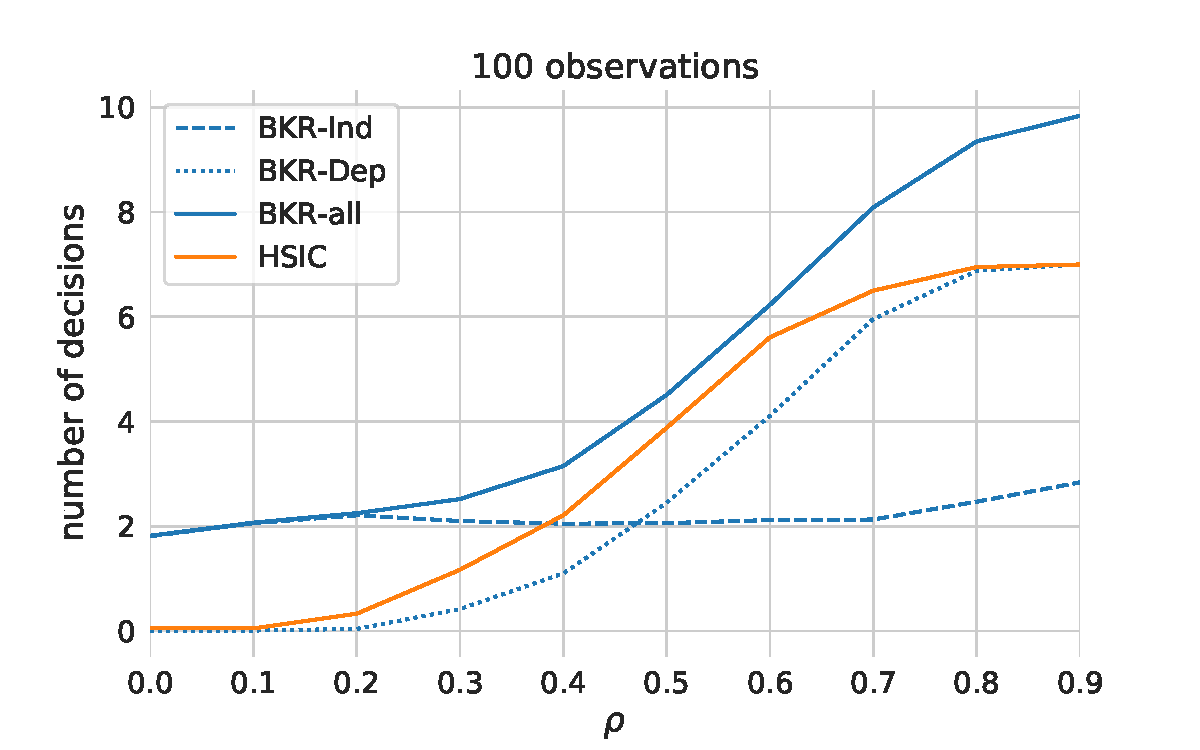
\includegraphics[height=1.9in]{100.pdf}
    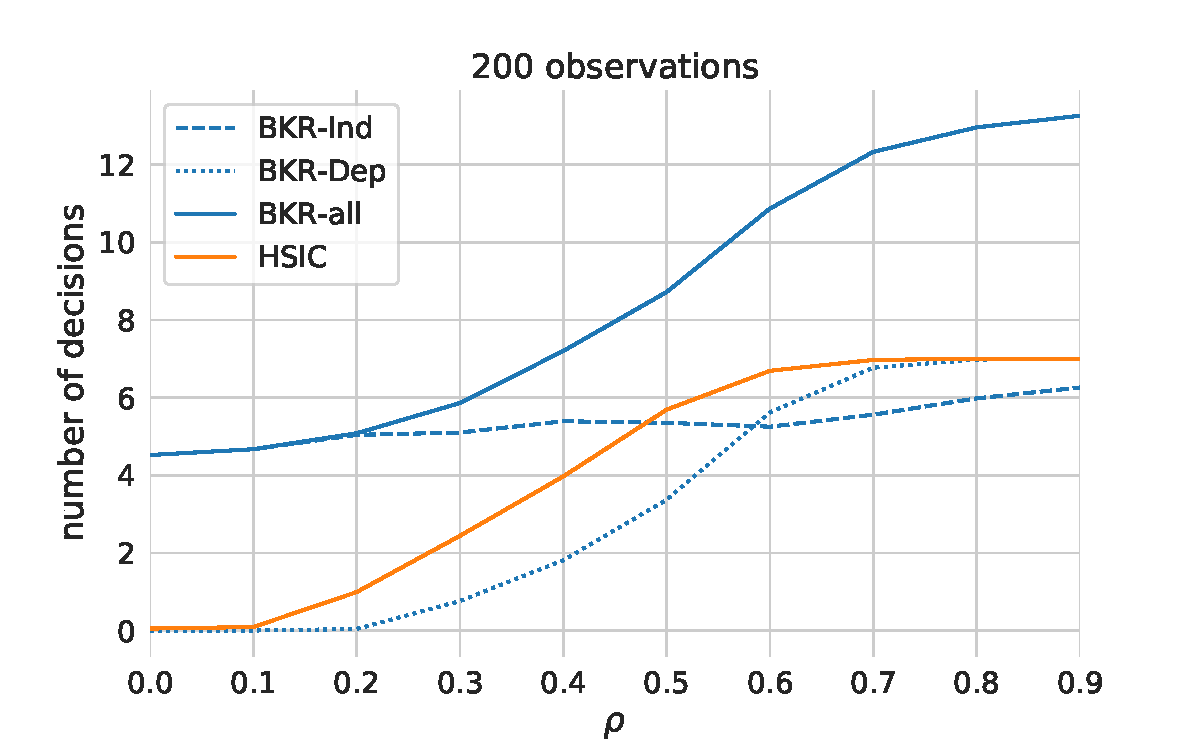
\includegraphics[height=1.9in]{200.pdf}
  \end{tabular}
  \caption{Synthetic dataset D1. \textbf{Just an example of figures.}}
  \label{fig:2}
\end{figure}


%%------------------------------------------------------------------------------
\section{Other Information}
\label{sec:other}
%%------------------------------------------------------------------------------
\subsection{Data management}
Responsible data management is part of good research. To promote effective and efficient data management, data sharing and data reuse, we expect researchers to carefully manage data. Research data are the evidence that underpin the answer to research questions, and can be used to validate findings. Data can be quantitative information or qualitative statements collected by researchers in the course of their work by experimentation, observation, modelling, interview or other methods, or information derived from existing evidence.

We understand software as included in the definition of research data. Algorithms, scripts and code developed by researchers in the course of their work may be necessary to access and interpret data. In such cases, the data management plan will be expected to address how information about such items will be made available.

Research results should be stored in such a way that they can be retrieved and reproduced and/or reused in the long term, also by researchers in disciplines and organisations other than those in which the research took place. The operating principle is that all stored data are, in principle, freely accessible and that access is only limited if needed for reasons such as privacy, public security, ethical restrictions, property rights and commercial interests. Any tools or software (algorithms, scripts and code developed by researchers in the course of their work) necessary to access and interpret data should be made available alongside the data.

\begin{enumerate}
  \item Will this project involve re-using existing research data?
        \begin{itemize}
          \item Yes: Are there any constraints on its re-use?
          \item No: Have you considered re-using existing data but discarded the possibility? Why?
        \end{itemize}

  \item Will data be collected or generated that are suitable for reuse?
        \begin{itemize}
          \item Yes: Please answer question 3.
          \item No: Please explain why the research will not result in reusable data or in data that cannot be stored or data that for other reasons are not relevant for reuse.
        \end{itemize}

  \item After the project has been completed, how will the data be stored for the long-term and made available for the use by third parties? Are there possible restrictions to data sharing or embargo reasons? Please state these here.
\end{enumerate}

%%------------------------------------------------------------------------------
\subsection{Motivation for choice of research group / supervisor / company}

This subsection can be used to explain why you have chosen this project with respect to supervisor, group and company. It is used to explain your view on the alignment of topic and the project team.

Note that the importance of each section and subsection and their respective content and size may vary from proposal to proposal. So you are expected to balance the content and length of each part accordingly. Typically Section~\ref{sec:other} is considerably smaller than the other sections. Often Sections~\ref{sec:goals}, \ref{sec:approach}, and~\ref{sec:evidence} are the largest sections.

\bibliographystyle{abbrv}
\bibliography{references}

\appendix
\section{Appendix}

You may provide any type of material as appendix to your project proposal. Typical appendices include additional details about the methodology, further pilot studies for illustration and demonstration of feasibility, images and results that were created, pointers to code (or pseudo-code itself), pointers to data, etc. There is no limit in the length of the appendices. For example, this appendix contain Table~\ref{table:somethinginside}, which has information that are not relevant but shows how to use a table here.

\begin{table}[ht]
  \caption{Some results of something. It is recommend not to try to understand it.\label{table:somethinginside}}
  \begin{center}
    \begin{tabular}{cccc|cc|cc}
              &                &           &       & \multicolumn{2}{c|}{Median} & \multicolumn{2}{c}{Maximum}                       \\
      Problem & Description    & Max Value & Nodes & Memory                      & Time(s)                     & Memory    & Time(s) \\
      \hline
      MINAP   & naive Bayes w/ & $10^{6}$  & 50    & $59$                        & $0.06$                      & $84$      & $0.08$  \\
              & random params  &           & 100   & $125$                       & $0.198$                     & $200$     & $0.285$ \\
              &                &           & 200   & $396$                       & $1.328$                     & $1238$    & $1.893$ \\
              &                &           & 300   & $1103$                      & $2.793$                     & $20863$   & $9.893$ \\
      MAP     & naive Bayes w/ & $10^{6}$  & 50    & $5$                         & $0.01$                      & $7$       & $0.015$ \\
              & random params  &           & 100   & $5$                         & $0.017$                     & $6$       & $0.023$ \\
              &                &           & 200   & $5$                         & $0.04$                      & $7$       & $0.047$ \\
              &                &           & 300   & $5$                         & $0.043$                     & $7$       & $0.049$ \\
      MINAP   & partition      & $10^{4}$  & 10    & $512$                       & $0.034$                     & $512$     & $0.039$ \\
              & problem        &           & 20    & $91857$                     & $11.553$                    & $100842$  & $17.42$ \\
              &                &           & 30    & $236979$                    & $77.09$                     & $264638$  & $82.81$ \\
              &                & $10^{5}$  & 10    & $512$                       & $0.036$                     & $512$     & $0.045$ \\
              &                &           & 20    & $347065$                    & $27.599$                    & $372670$  & $31.10$ \\
              &                &           & 30    & $2046264$                   & $532.318$                   & $2237859$ & $586.4$ \\
              &                & $10^{6}$  & 10    & $512$                       & $0.035$                     & $512$     & $0.038$ \\
              &                &           & 20    & $501347$                    & $34.672$                    & $510413$  & $38.13$ \\
              &                &           & 30    & $>10$Mln                    & $>600$                      & $>10$Mln  & $>600$  \\
      MINAP   & random struct. & $10^{6}$  & 50    & $57$                        & $0.046$                     & $101$     & $0.073$ \\
              & and parameters &           & 100   & $143$                       & $0.21$                      & $197$     & $0.326$ \\
              &                &           & 200   & $417$                       & $1.288$                     & $713$     & $1.761$ \\
              &                &           & 300   & $1129$                      & $2.509$                     & $10403$   & $14.53$ \\
      MAP     & random struct. & $10^{6}$  & 50    & $5$                         & $0.009$                     & $7$       & $0.014$ \\
              & and parameters &           & 100   & $5$                         & $0.018$                     & $6$       & $0.023$ \\
              &                &           & 200   & $5$                         & $0.042$                     & $7$       & $0.047$ \\
              &                &           & 300   & $6$                         & $0.049$                     & $7$       & $0.061$ \\
      \hline
    \end{tabular}
  \end{center}
\end{table}

\lipsum[1-4]

\end{document}



\end{document}
